\documentclass[10pt]{article}  

%%%%%%%% PREÁMBULO %%%%%%%%%%%%
\title{Plantilla para prácticas de UGR}
\usepackage[spanish]{babel} %Indica que escribiermos en español
\usepackage[utf8]{inputenc} %Indica qué codificación se está usando ISO-8859-1(latin1)  o utf8  
\usepackage{amsmath} % Comandos extras para matemáticas (cajas para ecuaciones,
% etc)
\usepackage{amssymb} % Simbolos matematicos (por lo tanto)
\usepackage{graphicx} % Incluir imágenes en LaTeX
\usepackage{color} % Para colorear texto
\usepackage{subfigure} % subfiguras
\usepackage{float} %Podemos usar el especificador [H] en las figuras para que se
% queden donde queramos
\usepackage{capt-of} % Permite usar etiquetas fuera de elementos flotantes
% (etiquetas de figuras)
\usepackage{sidecap} % Para poner el texto de las imágenes al lado
	\sidecaptionvpos{figure}{c} % Para que el texto se alinie al centro vertical
\usepackage{caption} % Para poder quitar numeracion de figuras
\usepackage{commath} % funcionalidades extras para diferenciales, integrales,
% etc (\od, \dif, etc)
\usepackage{cancel} % para cancelar expresiones (\cancelto{0}{x})

\graphicspath{{/Users/jesusgarciamanday/Desktop/Master/CC-II/Practicas/Practica1/p1/Imagenes/}}

\usepackage{anysize} 					% Para personalizar el ancho de  los márgenes
\marginsize{2cm}{2cm}{2cm}{2cm} % Izquierda, derecha, arriba, abajo

\usepackage{appendix}
\renewcommand{\appendixname}{Apéndices}
\renewcommand{\appendixtocname}{Apéndices}
\renewcommand{\appendixpagename}{Apéndices} 

% Para que las referencias sean hipervínculos a las figuras o ecuaciones y
% aparezcan en color
\usepackage[colorlinks=true,plainpages=true,citecolor=blue,linkcolor=blue]{hyperref}
%\usepackage{hyperref} 
% Para agregar encabezado y pie de página
\usepackage{fancyhdr} 
\pagestyle{fancy}
\fancyhf{}
\fancyhead[L]{\footnotesize UGR} %encabezado izquierda
\fancyhead[R]{\footnotesize CCIA}   % dereecha
\fancyfoot[R]{\footnotesize Pr\'actica 1 - OpenNebula }  % Pie derecha
\fancyfoot[C]{\thepage}  % centro
\fancyfoot[L]{\footnotesize Master en Ingenier\'ia Inform\'atica }  %izquierda
\renewcommand{\footrulewidth}{0.4pt}


\usepackage{listings} % Para usar código fuente
\definecolor{dkgreen}{rgb}{0,0.6,0} % Definimos colores para usar en el código
\definecolor{gray}{rgb}{0.5,0.5,0.5} 
% configuración para el lenguaje que queramos utilizar
\lstset{language=Matlab,
   keywords={break,case,catch,continue,else,elseif,end,for,function,
      global,if,otherwise,persistent,return,switch,try,while},
   basicstyle=\ttfamily,
   keywordstyle=\color{blue},
   commentstyle=\color{red},
   stringstyle=\color{dkgreen},
   numbers=left,
   numberstyle=\tiny\color{gray},
   stepnumber=1,
   numbersep=10pt,
   backgroundcolor=\color{white},
   tabsize=4,
   showspaces=false,
   showstringspaces=false}

\newcommand{\sen}{\operatorname{\sen}}	% Definimos el comando \sen para el seno
%en español

\title{Práctica 1 - OpenNebula}

%%%%%%%% TERMINA PREÁMBULO %%%%%%%%%%%%

\begin{document}

%%%%%%%%%%%%%%%%%%%%%%%%%%%%%%%%%% PORTADA %%%%%%%%%%%%%%%%%%%%%%%%%%%%%%%%%%%%%%%%%%%%
																					%%%
\begin{center}																		%%%
\newcommand{\HRule}{\rule{\linewidth}{0.5mm}}									%%%\left
 																					%%%
\begin{minipage}{0.48\textwidth} \begin{flushleft}
%
\includegraphics[scale = 0.63]{Imagenes/logo_upiita}
\end{flushleft}\end{minipage}
\begin{minipage}{0.48\textwidth} \begin{flushright}
%
\includegraphics[scale = 0.35]{Imagenes/IPN}
\end{flushright}\end{minipage}

													 								%%%
\vspace*{-1.5cm}								%%%
																					%%%	
\textsc{\huge Universidad de\\ \vspace{5px} Granada}\\[1.5cm]	

\textsc{\LARGE Master Profesional en Ingenier\'ia Inform\'atica }\\[1.5cm]													%%%

\begin{minipage}{0.9\textwidth} 
\begin{center}																					%%%
\textsc{\LARGE Pr\'actica 1}
\end{center}
\end{minipage}\\[0.5cm]
%%%
    																				%%%
 			\vspace*{1cm}																		%%%
																					%%%
\HRule \\[0.4cm]																	%%%
{ \huge \bfseries OpenNebula}\\[0.4cm]	%%%
 																					%%%
\HRule \\[1.5cm]																	%%%
 																				%%%
																					%%%
\begin{minipage}{0.46\textwidth}													%%%
\begin{flushleft} \large															%%%
\emph{Autor:}\\	
Manuel Jes\'us Garc\'ia Manday (nickter@correo.ugr.es)\\
%%%
			%\vspace*{2cm}	
            													%%%
										 						%%%
\end{flushleft}																		%%%
\end{minipage}		
																%%%
\begin{minipage}{0.52\textwidth}		
\vspace{-0.6cm}											%%%
\begin{flushright} \large															%%%
													%%%
\end{flushright}																	%%%
\end{minipage}	
\vspace*{1cm}
%\begin{flushleft}
 	
%\end{flushleft}
%%%
 		\flushleft{\textbf{\Large Master en Ingenier\'ia Inform\'atica}	}\\																		%%%
\vspace{2cm} 																				
\begin{center}																					
{\large 20 de abril de 2017}																	%%%
 			\end{center}												  						
\end{center}							 											
																					
\newpage																		
%%%%%%%%%%%%%%%%%%%% TERMINA PORTADA %%%%%%%%%%%%%%%%%%%%%%%%%%%%%%%%

\tableofcontents 

\newpage

\section{Objetivo.}
El objetivo de esta práctica es familiarizarse con el uso de una plataforma IaaS y desarrollar habilidades de despliegue de máquinas virtuales y aplicaciones web sencillas.\\


\section{Configuración de la MV1 (con servidor Web).} 
Para poder configurar las máquinas virtuales creadas anteriormente es necesario establecer una conexión remota con ellas, por lo que se necesita conocer la dirección ip que se les ha sido asginada. En esta sección vamos a configurar la primera máquina virtual, es decir, la que tendrá el servicio web. Como se acaba de mencionar se necesita la dirección ip de la máquina virtual para realizar la conexión remota, y para ello existe un comando que nos muestra la información detallada de la máquina virtual en funcionamiento. Ejecutando \textbf{onevm show} acompañado del \textbf{ID} de la máquina virtual obtendremos la información de la misma como se muestra a continuación: \\

\begin{figure}[H]
	\begin{center}
 		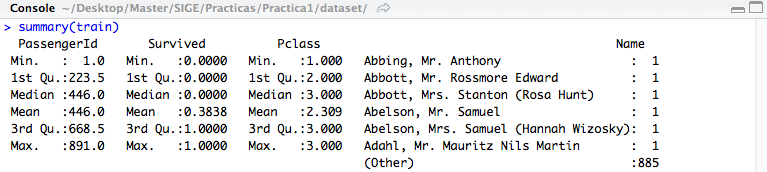
\includegraphics[width = 0.75\textwidth]{p1-img11}
 		\captionof{figure}{\label{fig:IPN}Información de la primera máquina virtual (I).} 
	\end{center} 
\end{figure}

\begin{figure}[H]
	\begin{center}
 		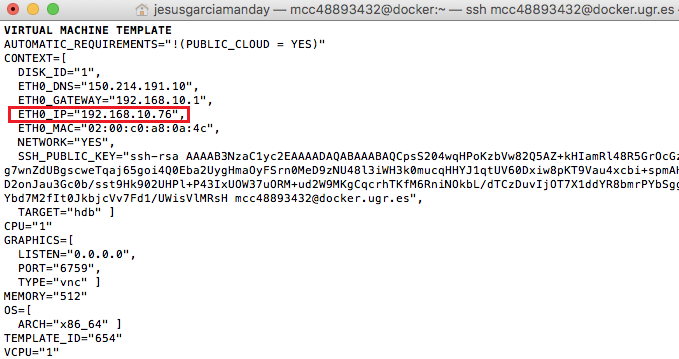
\includegraphics[width = 0.75\textwidth]{p1-img12}
 		\captionof{figure}{\label{fig:IPN}Información de la primera máquina virtual (II).} 
	\end{center} 
\end{figure}


De toda la información arrojada la que ahora mismo nos interesa es la que se indica con \textbf{ETH0\_IP}, que es donde se encuentra la dirección ip que se le ha asignado a dicha máquina virtual. Una vez que ya se conoce la dirección ip de la máquina nos conectamos a ella para comenzar con la configuración de la misma.\\

\begin{figure}[H]
	\begin{center}
 		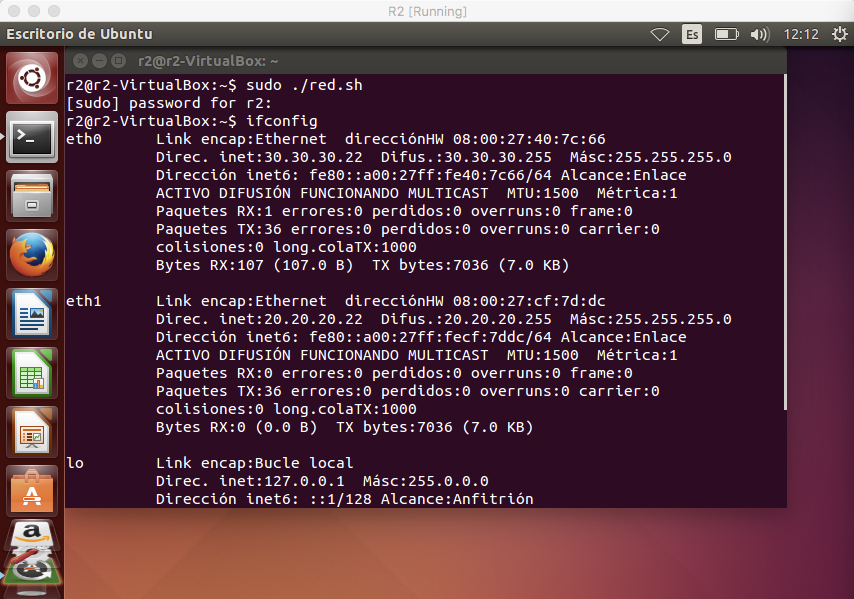
\includegraphics[width = 0.75\textwidth]{p1-img13}
 		\captionof{figure}{\label{fig:IPN}Conexión remota con la primera máquina virtual.} 
	\end{center} 
\end{figure}

\begin{figure}[H]
	\begin{center}
 		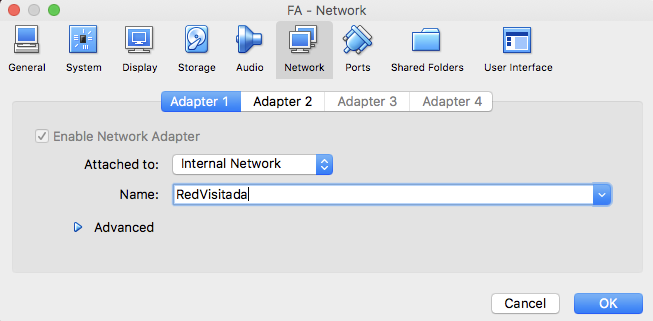
\includegraphics[width = 0.75\textwidth]{p1-img14}
 		\captionof{figure}{\label{fig:IPN}Actualización del sistema.} 
	\end{center} 
\end{figure}

\begin{figure}[H]
	\begin{center}
 		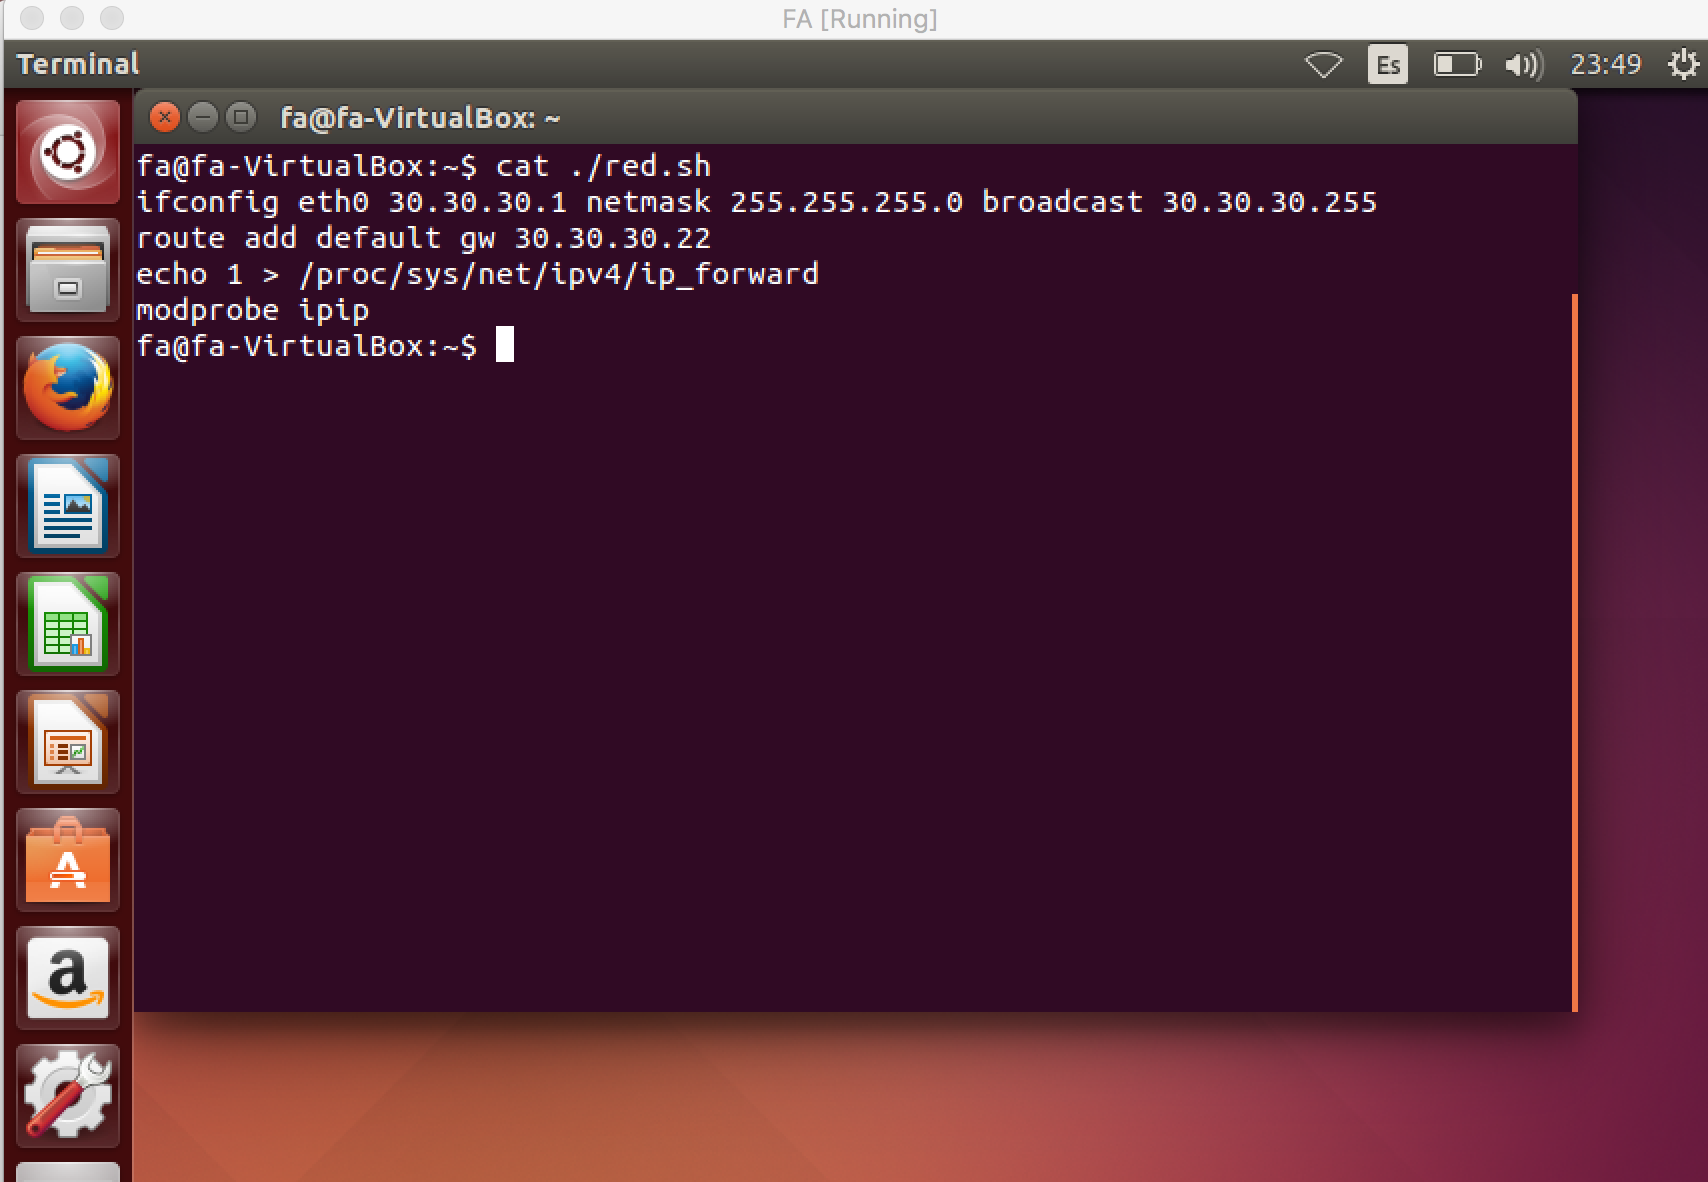
\includegraphics[width = 0.75\textwidth]{p1-img15}
 		\captionof{figure}{\label{fig:IPN}Instalación de los servicios \textbf{Apache}. y \textbf{PHP} (I)} 
	\end{center} 
\end{figure}

\begin{figure}[H]
	\begin{center}
 		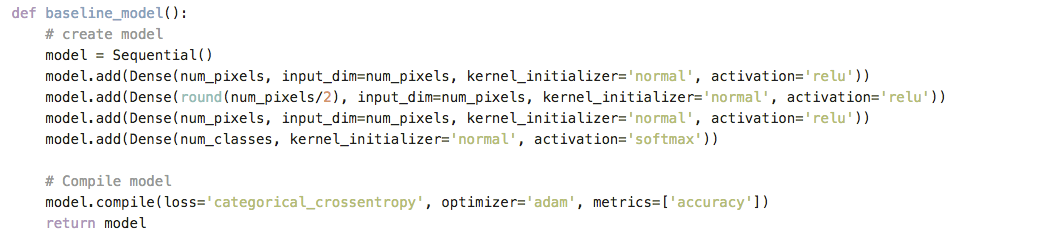
\includegraphics[width = 0.75\textwidth]{p1-img16}
 		\captionof{figure}{\label{fig:IPN}Instalación de los servicios \textbf{Apache}. y \textbf{PHP5} (II)} 
	\end{center} 
\end{figure}

En las siguientes imágenes se puede ver como ambos servicios se han instalado correctamente en la máquina virtual, quedando totalmente configurada. \\

\begin{figure}[H]
	\begin{center}
 		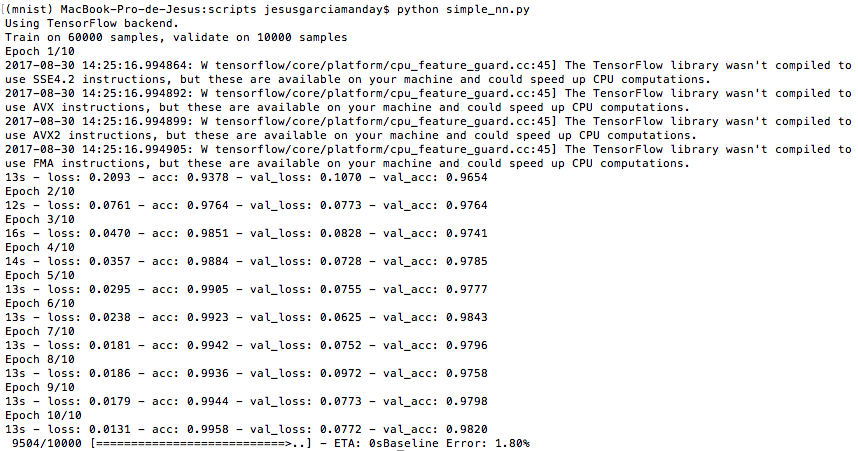
\includegraphics[width = 0.75\textwidth]{p1-img17}
 		\captionof{figure}{\label{fig:IPN}Comprobando instalación \textbf{Apache}} 
	\end{center} 
\end{figure}

\begin{figure}[H]
	\begin{center}
 		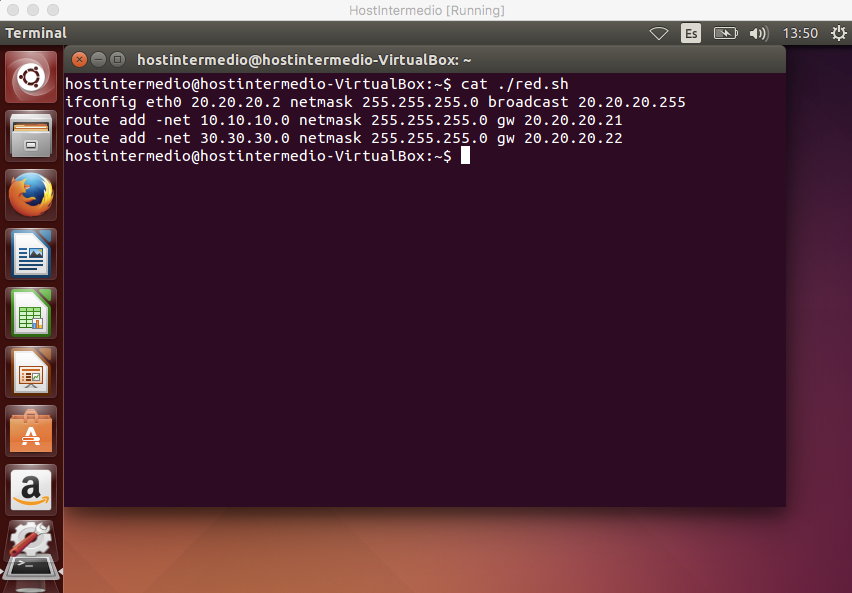
\includegraphics[width = 0.75\textwidth]{p1-img18}
 		\captionof{figure}{\label{fig:IPN}Comprobando instalación \textbf{PHP5} (II)} 
	\end{center} 
\end{figure}


\section{Configuración de la MV2 (con SGBD).} 
Con la primera máquina virtual ya configurada, hacemos lo propio con la segunda. Repetimos el mismo paso que se hizo en el apartado anterior para conocer la dirección ip de la segunda máquina virtual, por lo que volvemos a ejecutar el comando \textbf{onevm show 860} referido al identificador de esta máquina.\\

\begin{figure}[H]
	\begin{center}
 		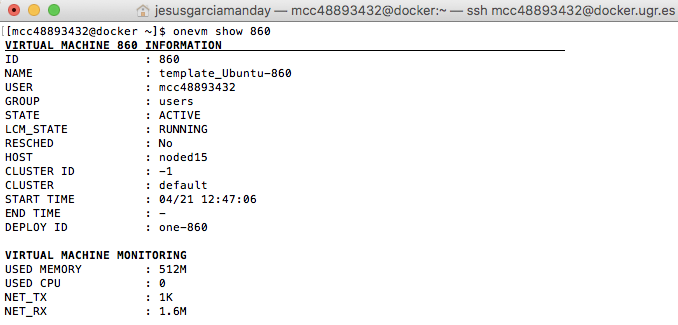
\includegraphics[width = 0.75\textwidth]{p1-img19}
 		\captionof{figure}{\label{fig:IPN}Información de la segunda máquina virtual (I).} 
	\end{center} 
\end{figure}

\begin{figure}[H]
	\begin{center}
 		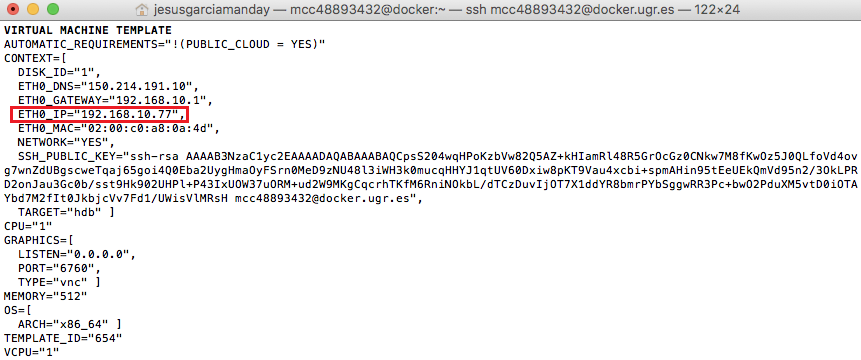
\includegraphics[width = 0.75\textwidth]{p1-img20}
 		\captionof{figure}{\label{fig:IPN}Información de la segunda máquina virtual (II).} 
	\end{center} 
\end{figure}

Conocida ya la dirección ip de esta segunda máquina virtual, lo siguiente es establecer una conexión remota a ella para configurarla con los servicios necesarios.\\

\begin{figure}[H]
	\begin{center}
 		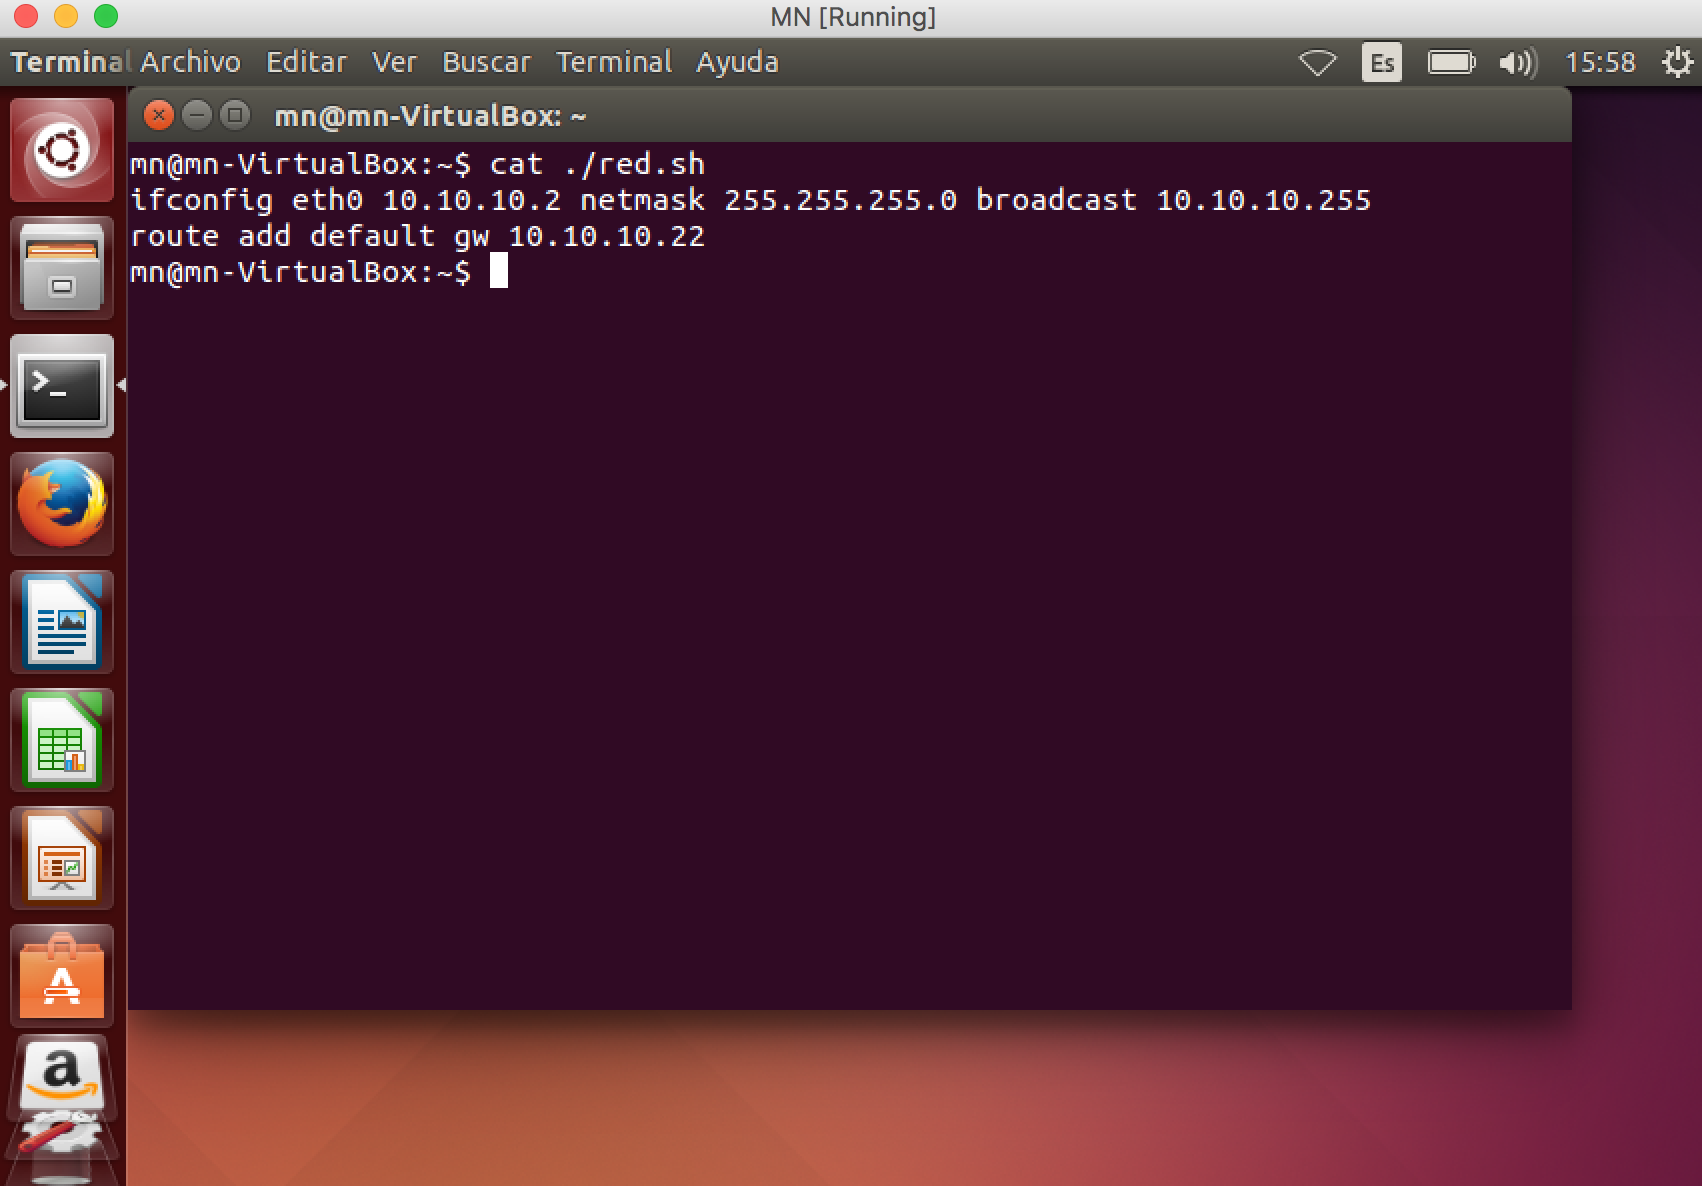
\includegraphics[width = 0.75\textwidth]{p1-img21}
 		\captionof{figure}{\label{fig:IPN}Conexión remota con la segunda máquina virtual.} 
	\end{center} 
\end{figure}

\begin{figure}[H]
	\begin{center}
 		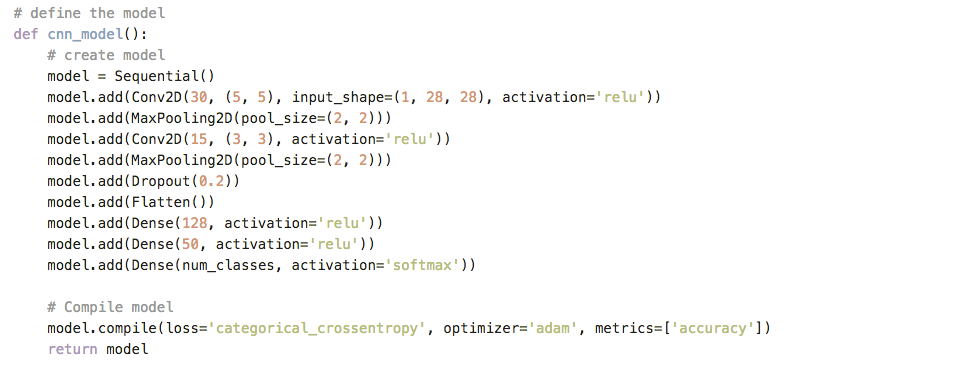
\includegraphics[width = 0.75\textwidth]{p1-img22}
 		\captionof{figure}{\label{fig:IPN}Actualización del sistema.} 
	\end{center} 
\end{figure}

\begin{figure}[H]
	\begin{center}
 		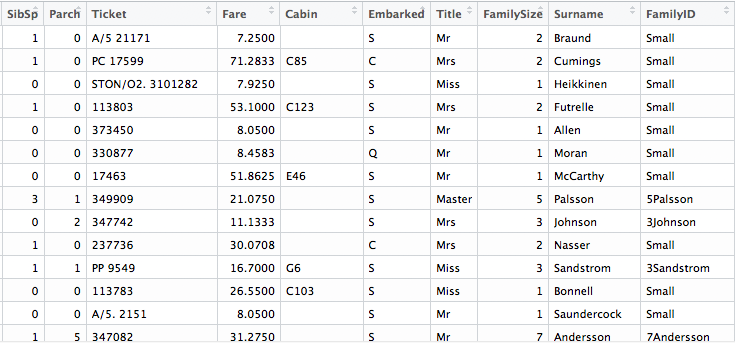
\includegraphics[width = 0.75\textwidth]{p1-img23}
 		\captionof{figure}{\label{fig:IPN}Instalación del servicio \textbf{MySQL} (I)} 
	\end{center} 
\end{figure}

\begin{figure}[H]
	\begin{center}
 		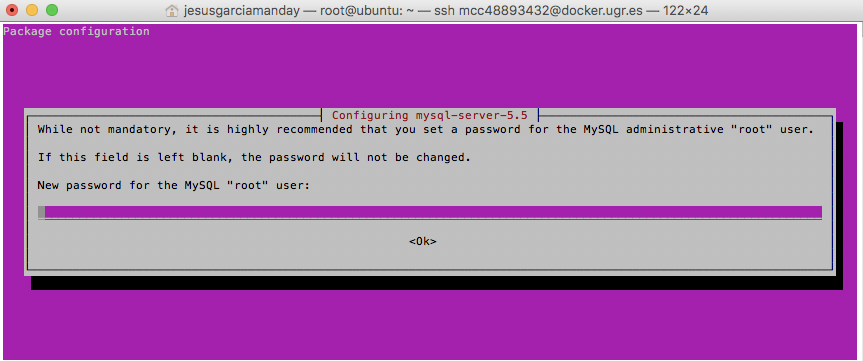
\includegraphics[width = 0.75\textwidth]{p1-img24}
 		\captionof{figure}{\label{fig:IPN}Instalación del servicio \textbf{MySQL} (II)} 
	\end{center} 
\end{figure}

\begin{figure}[H]
	\begin{center}
 		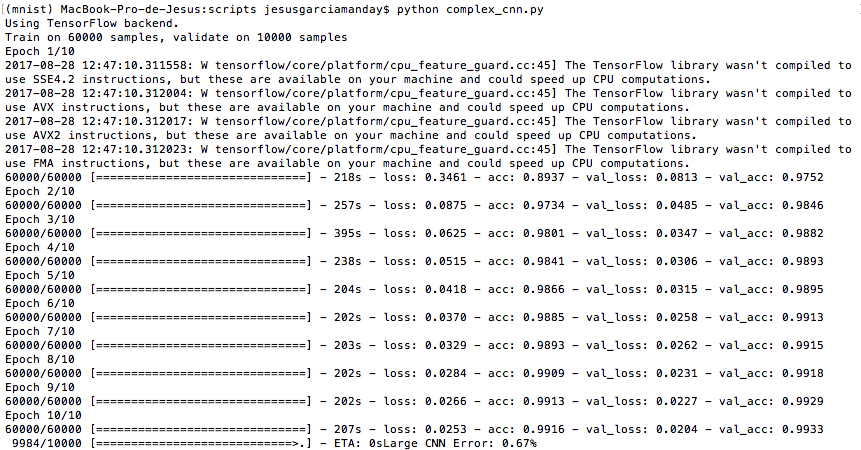
\includegraphics[width = 0.75\textwidth]{p1-img25}
 		\captionof{figure}{\label{fig:IPN}Comprobación del servicio \textbf{MySQL}} 
	\end{center} 
\end{figure}



\section{Descripción de la aplicación web. Objetivo, funcionalidad, arquitectura software, base de datos, tablas.}
La aplicación que se va a estar ejecutando en la primera máquina virtual con el servicio Web \textbf{Apache} es una aplicación de gestión de usuarios que muestra una lista de los mismos y que permite las operaciones de insertar y eliminar usuarios de la base de datos que se encuentra en la segunda máquina virtual con el servicio de \textbf{MySQL}.\\

La arquitectura de la aplicación esta basada en microservicios, en este caso son dos los principales software sobre los que se sustenta dicha aplicación (\textbf{Apache} y \textbf{MySQL}). Cada uno de los servicios mencionados residen en una máquina virtual diferente, comunicandose de forma remota entre ellos a través de protocolos de internet como http, icmp y tcp entre otros. En la siguiente imagen se puede apreciar la arquitectura en la que está basada la aplicación web.\\ \\

 \begin{figure}[H]
	\begin{center}
 		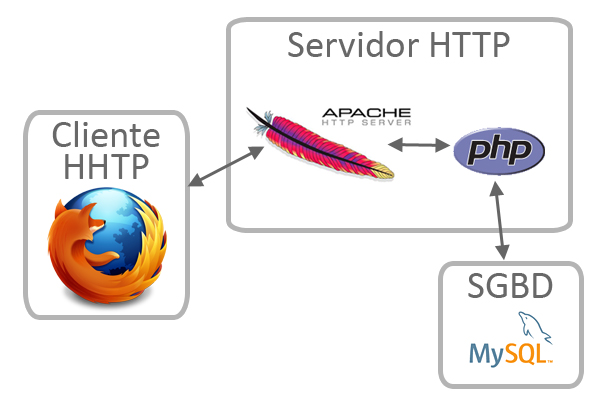
\includegraphics[width = 0.75\textwidth]{p1-img26}
 		\captionof{figure}{\label{fig:IPN}Arquitectura de la aplicación.} 
	\end{center} 
\end{figure}

En la primera máquina virtual es donde se aloja el servidor Web de \textbf{Apache} y es por tanto donde se han definido los ficheros \textbf{php} que manejan las acciones realizadas por el usuario sobre la aplicación. Son tres los ficheros que se han implementado para el servidor los cuales residen en la dirección \textbf{/var/www/html} del mismo. El fichero por defecto que se ejecuta al acceder a la página inicial del servidor es el \textbf{index.php}, existen dos ficheros más que se encargan de cada una de las dos operaciones permitidas en la aplicación, la insercción de un nuevo usuario a través del fichero \textbf{insert\_user.php} y elminar a un usuario existente mediante el fichero \textbf{delete\_user.php}. En las siguientes imagenes se muestra la estructura y el contenido de dichos ficheros.\\ 

 \begin{figure}[H]
	\begin{center}
 		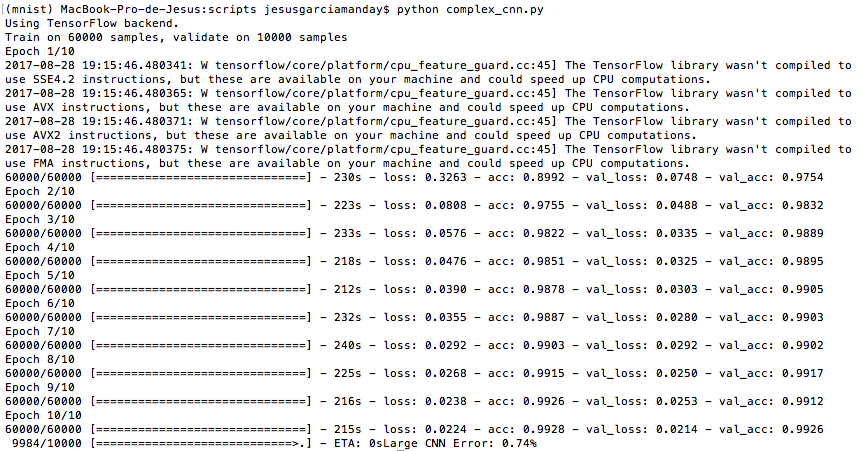
\includegraphics[width = 0.75\textwidth]{p1-img27}
 		\captionof{figure}{\label{fig:IPN}Fichero index.php (I).} 
	\end{center} 
\end{figure}

 \begin{figure}[H]
	\begin{center}
 		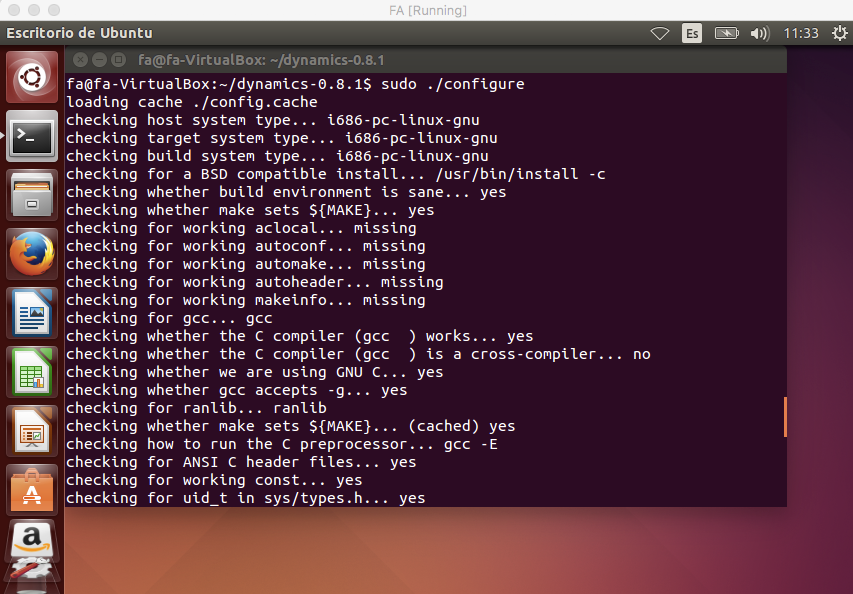
\includegraphics[width = 0.75\textwidth]{p1-img28}
 		\captionof{figure}{\label{fig:IPN}Fichero index.php (II).} 
	\end{center} 
\end{figure}

 \begin{figure}[H]
	\begin{center}
 		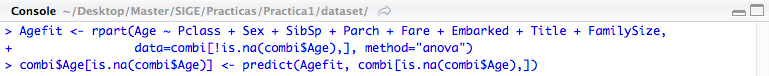
\includegraphics[width = 0.75\textwidth]{p1-img29}
 		\captionof{figure}{\label{fig:IPN}Fichero index.php (III).} 
	\end{center} 
\end{figure}

 \begin{figure}[H]
	\begin{center}
 		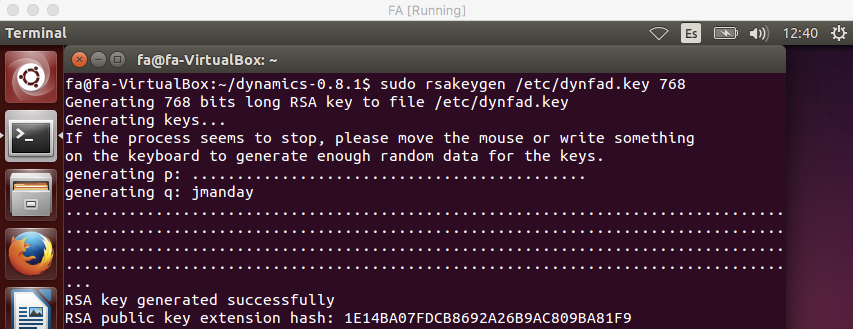
\includegraphics[width = 0.75\textwidth]{p1-img30}
 		\captionof{figure}{\label{fig:IPN}Fichero index.php (IV).} 
	\end{center} 
\end{figure}

 \begin{figure}[H]
	\begin{center}
 		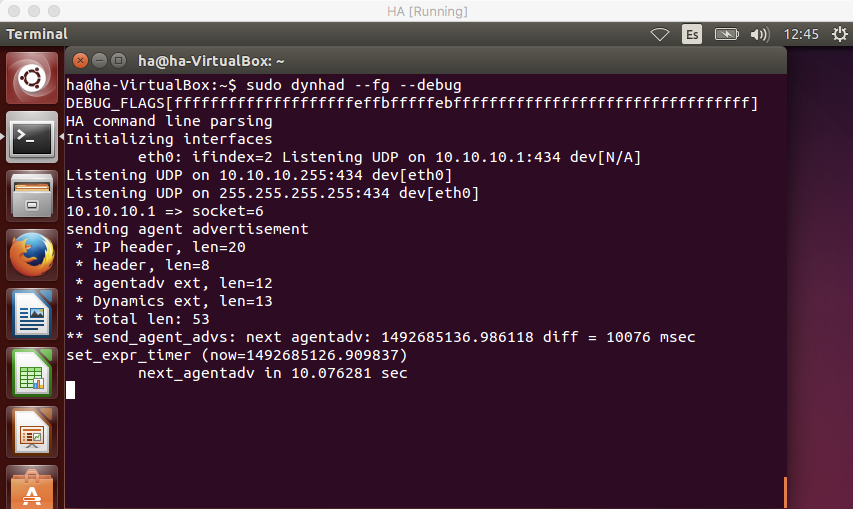
\includegraphics[width = 0.75\textwidth]{p1-img31}
 		\captionof{figure}{\label{fig:IPN}Fichero index.php (V).} 
	\end{center} 
\end{figure}

 \begin{figure}[H]
	\begin{center}
 		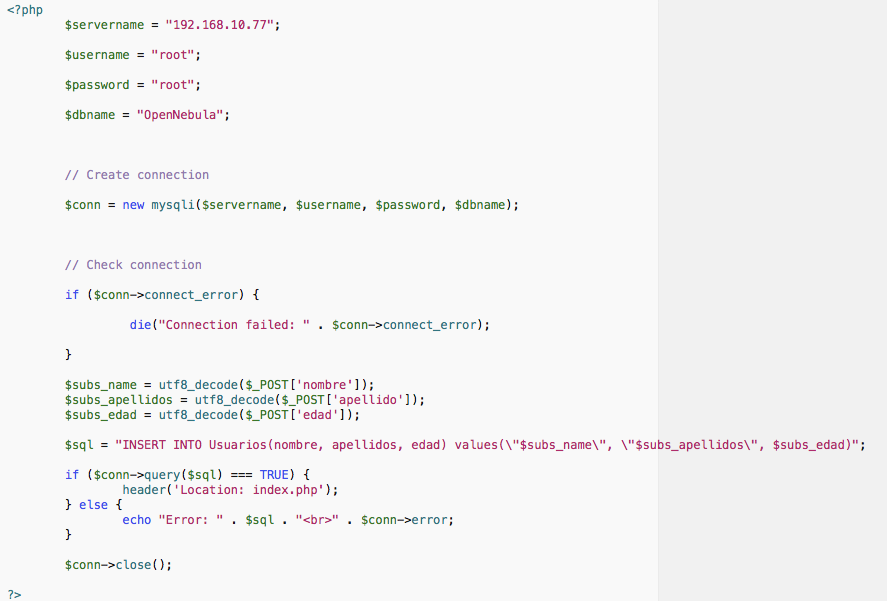
\includegraphics[width = 0.75\textwidth]{p1-img32}
 		\captionof{figure}{\label{fig:IPN}Fichero insert\_user.php .} 
	\end{center} 
\end{figure}

 \begin{figure}[H]
	\begin{center}
 		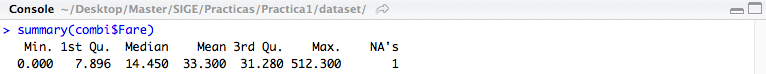
\includegraphics[width = 0.75\textwidth]{p1-img33}
 		\captionof{figure}{\label{fig:IPN}Fichero delete\_user.php .} 
	\end{center} 
\end{figure}

En la segunda máquina virtual es donde reside el SGBD \textbf{MySQL} y por lo tanto es donde se ha creado la base de datos correspondiente sobre la que trabaja la aplicación. En dicha base de datos se ha creado la tabla \textbf{Usuarios}, la cual va a representar el modelo de datos para almacenar la información referente a los usuarios que se añadan o eliminen desde la aplicación. En las imagenes de a continuación se muestra la conexión hacia dicha máquina virtual así como el uso de la base de datos, la creación de la tabla y la insercción de algunos registros.\\


 \begin{figure}[H]
	\begin{center}
 		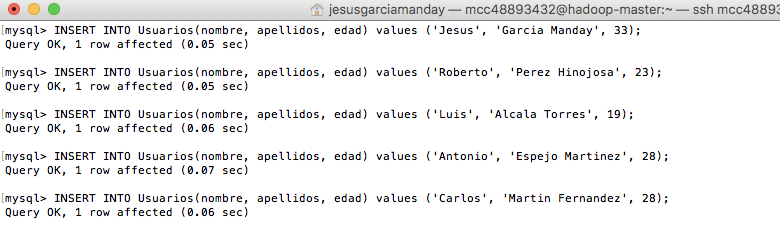
\includegraphics[width = 0.75\textwidth]{p1-img34}
 		\captionof{figure}{\label{fig:IPN}Insertando registros en la base de datos.} 
	\end{center} 
\end{figure} 


El resultado final de la aplicación lo podemos apreciar en la imagen de abajo.\\

 \begin{figure}[H]
	\begin{center}
 		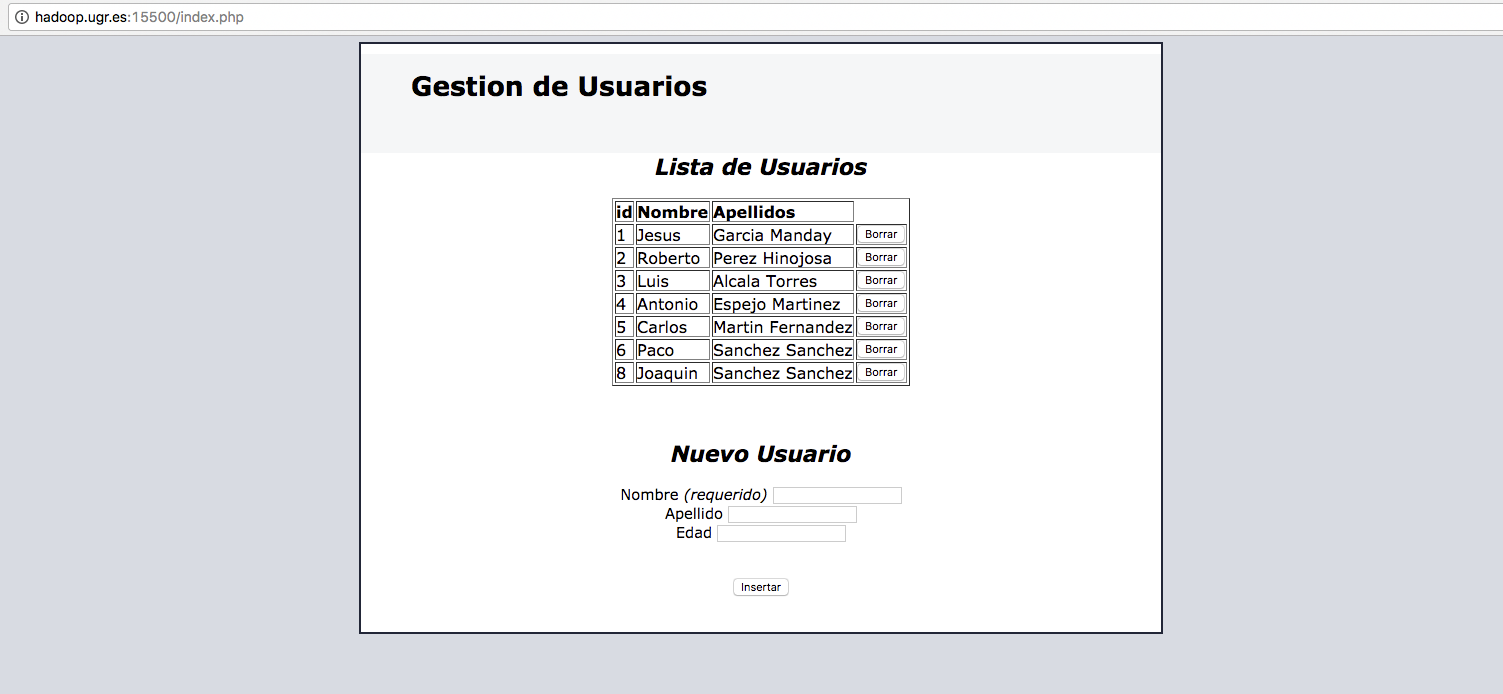
\includegraphics[width = 0.75\textwidth]{p1-img35}
 		\captionof{figure}{\label{fig:IPN}Aplicación web.} 
	\end{center} 
\end{figure}



\section{Breve manual de despliegue de las MVs.} 

Lo primero que se debe realizar es una conexión remota mediante el comando \textbf{ssh mcc48893432@docker.ugr.es} hacia el servidor docker.ugr.es donde se encuentra instalado el sistema \textbf{OpenNebula}. Una vez establecida la conexión, con la siguiente orden nos conectamos al sistema para poder trabajar con el. \\

\begin{figure}[H]
	\begin{center}
 		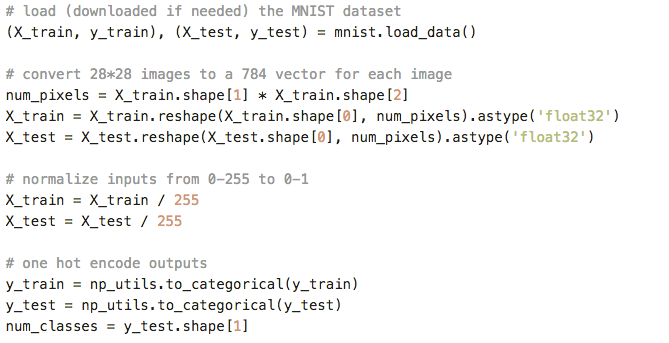
\includegraphics[width = 0.75\textwidth]{p1-img1}
 		\captionof{figure}{\label{fig:IPN}Conexión ssh y acceso al sistema OpenNebula.} 
	\end{center} 
\end{figure}

Con la sesión iniciada correctamente en \textbf{OpenNebula}, pasamos a ver las imágenes de los sitemas operativos que hay disponibles en dicho sistema para crear las dos máquinas virtuales necesarias  a través del comando \textbf{oneimage list}.\\

\begin{figure}[H]
	\begin{center}
 		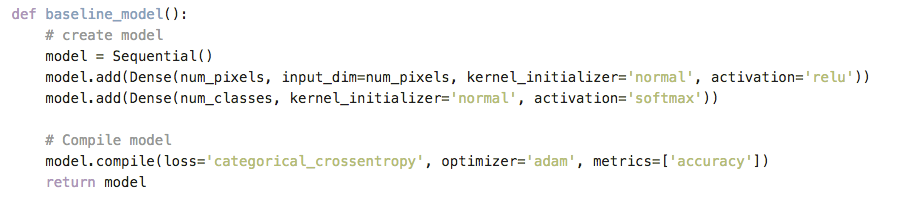
\includegraphics[width = 0.75\textwidth]{p1-img2}
 		\captionof{figure}{\label{fig:IPN}Imágenes de sistemas operativos disponibles en OpenNebula.} 
	\end{center} 
\end{figure}

Como se ha podido comprobar en la anterior imagen, \textbf{OpenNebula} dispone de varias imagenes de sistemas operativos que difieren según el ámbito para el que se vayan a emplear. Para nuestro caso nos bastará con una imagen de un sistema operativo tipo \textbf{CentOS} o \textbf{Ubuntu}. Antes de ponernos a definir y crear las máquinas virtuales es necesario comprobar que se tiene creada una red virtual para ser capaz de lanzar máquinas dentro de un espacio de direcciones ip correcto. Esto lo podemos comprobar ejecutando el comando \textbf{onevnet list}.\\

 \begin{figure}[H]
	\begin{center}
 		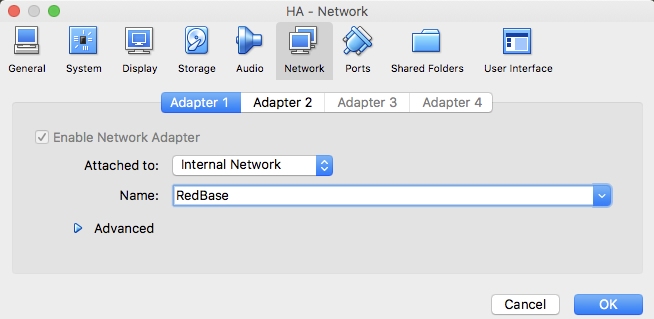
\includegraphics[width = 0.75\textwidth]{p1-img3}
 		\captionof{figure}{\label{fig:IPN}Comprobación de red virtual (I).} 
	\end{center} 
\end{figure}

\begin{figure}[H]
	\begin{center}
 		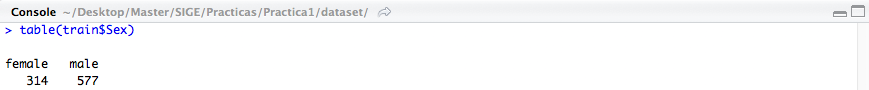
\includegraphics[width = 0.75\textwidth]{p1-img4}
 		\captionof{figure}{\label{fig:IPN}Comprobación de red virtual (II).} 
	\end{center} 
\end{figure}


En la \textbf{Figura 4} se puede apreciar como la red virtual con el ID \textbf{218} y el NAME \textbf{mcc48893432\_vnet} está correctamente creada para el usuario \textbf{mcc48893432}. Llegado a este punto toca definir la plantilla en base a la cual se crearán las dos máquinas virtuales necesarias, una para el despliegue de la aplicación y otra para la base de datos. Ambas se crearán a partir de la misma plantilla, ya que los recursos, prestaciones y características que necesitan son similares. Posteriormente se aprovisionarán y configurarán de manera individual a cada una de ellas con las herramientas y servicios necesarios en función del rol que tenga asignado. Con el comando \textbf{onetemplate create} definimos la plantilla en función de los parámetros que le indiquemos como se puede ver en la imagen de a continuación. \\ \\

\begin{figure}[H]
	\begin{center}
 		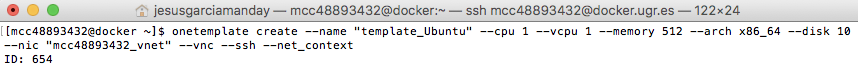
\includegraphics[width = 0.75\textwidth]{p1-img5}
 		\captionof{figure}{\label{fig:IPN}Creación de plantilla de máquina virtual.} 
	\end{center} 
\end{figure}

A la plantilla de máquina virtual creada se le ha dado el nombre de "template\_Ubuntu", a la cual se le asignará una cpu y otra virtual. Tendrá \textbf{512 MB} de memoria \textbf{RAM} y estará basada en una arquitectura \textbf{x86\_64}. Para el sistema operativo se ha seleccionada la imagen de un \textbf{Ubuntu 14.04}. La red virtual a la que va a pertenecer será la asginada este usuario (\textbf{mcc48893432\_vnet}) y comprobada anteriormente. También se le añade la opción de poder acceder de manera remota desde ssh. Ejecutamos el comando \textbf{onetemplate list} para comprobar que efectivamente se ha creado con éxito. \\

\begin{figure}[H]
	\begin{center}
 		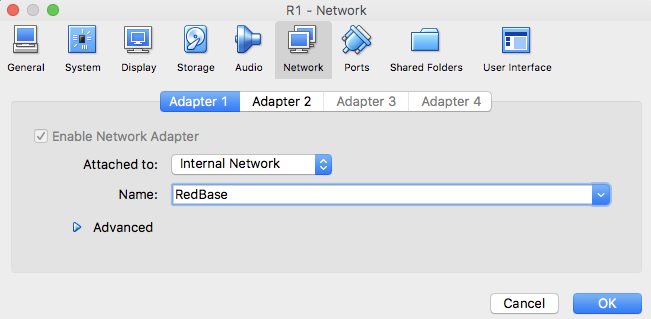
\includegraphics[width = 0.75\textwidth]{p1-img6}
 		\captionof{figure}{\label{fig:IPN}Listado de plantillas de máquinas virtuales.} 
	\end{center} 
\end{figure}

Una vez que se ha generado la plantilla de la máquina virtual, ya podemos comenzar con el despliegue de las dos máquinas virtuales. Para lanzar una instancia de una máquina virtual en base a una plantilla tenemos que ejecutar el comando \textbf{onetemplate instantiate} seguido del ID de la plantilla. Vamos a desplegar una primera máquina virtual que será la que contenga los servicios de \textbf{APACHE} y \textbf{PHP},  haciendo de servidor Web donde se alojará la aplicación.\\

\begin{figure}[H]
	\begin{center}
 		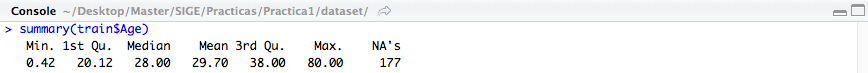
\includegraphics[width = 0.75\textwidth]{p1-img7}
 		\captionof{figure}{\label{fig:IPN}Despliegue de máquina virtual en base a una plantilla.} 
	\end{center} 
\end{figure}

En la \textbf{Figura 7} se puede apreciar el despliegue de una máquina virtual en base a una plantilla, y como éste devuelve un identificador (\textbf{859}) que hace referencia a la máquina virtual creada. Comprobemos que la máquina virtual con ese identificador se ha creado correctamente ejecutando el comando \textbf{onevm list}. \\

\begin{figure}[H]
	\begin{center}
 		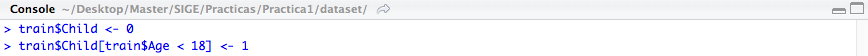
\includegraphics[width = 0.75\textwidth]{p1-img8}
 		\captionof{figure}{\label{fig:IPN}Comprobando que se ha creado la primera máquina virtual.} 
	\end{center} 
\end{figure}

Como se puede apreciar en la anterior imagen, la máquina virtual con el ID \textbf{859} se ha creado correctamente y se encuentra ejecutando, como muestra su estado \textbf{'running'}. Ahora vamos a desplegar otra instancia de máquina virtual en base a esa misma plantilla, la cual en esta ocasión será destinada al servicio de \textbf{MySQL}.\\

\begin{figure}[H]
	\begin{center}
 		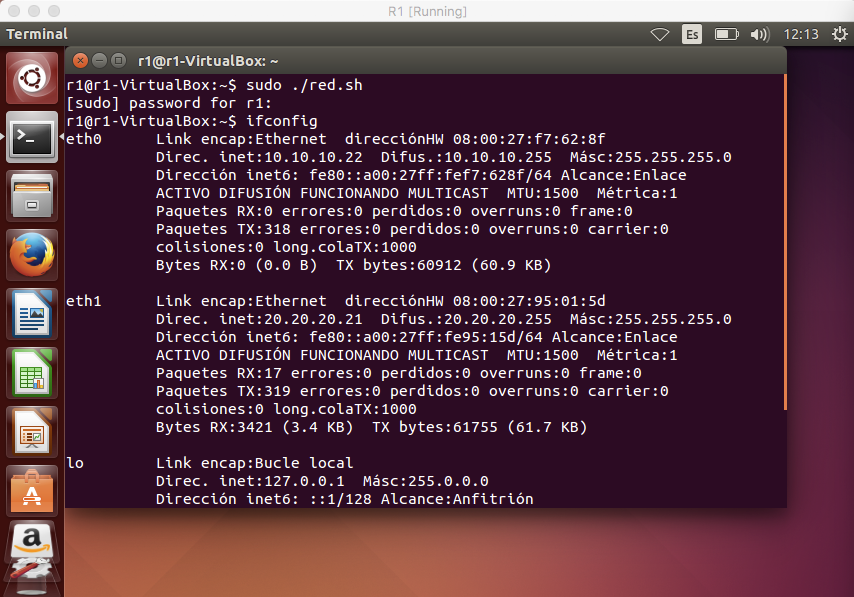
\includegraphics[width = 0.75\textwidth]{p1-img9}
 		\captionof{figure}{\label{fig:IPN}Despliegue de una segunfa máquina virtual en base a una plantilla.} 
	\end{center} 
\end{figure}

En la imagen de arriba vemos que el despligue de la segunda máquina virtual se ha realizado con éxito, ya que el sistema ha devuelto de identificador (\textbf{ID 860}) de la misma forma como sucedió con el despligue de la primera máquina virtual. Al igual que hicimos antes, vamos a comprobar cual es el estado de esta nueva máquin virtual con el indetificado \textbf{860} con ese mismo comando. \\

\begin{figure}[H]
	\begin{center}
 		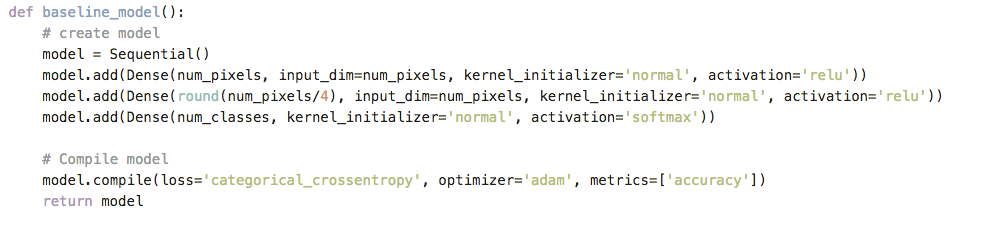
\includegraphics[width = 0.75\textwidth]{p1-img10}
 		\captionof{figure}{\label{fig:IPN}Comprobando que se ha creado la segunda máquina virtual.} 
	\end{center} 
\end{figure}


Se puede apreciar en la figura anterior que la segunda máquina virtual se ha desplegado correctamente y prueba de ello es el estado \textbf{'running'} que muestra al igual que la primera máquina virtual, lo que nos dice que ambas se encuentran ejecutando y listas para ser utilizadas.\\


\section{Breve manual de uso de la aplicación web.} 
Como ya se mencionó en el apartado de la \textbf{Descripción de la aplicación web}, este software es una simple aplicación de gestión usuarios a través de la cual es posible añadir usuarios o eliminar usuarios de una base de datos. Cuando se ejecuta la aplicación lo que nos muestra es la lista de usuarios que existen en ese momento en la base de datos, de los cuales nos muestra atributos como su identificador, su nombre y sus apellidos. \\

\begin{figure}[H]
	\begin{center}
 		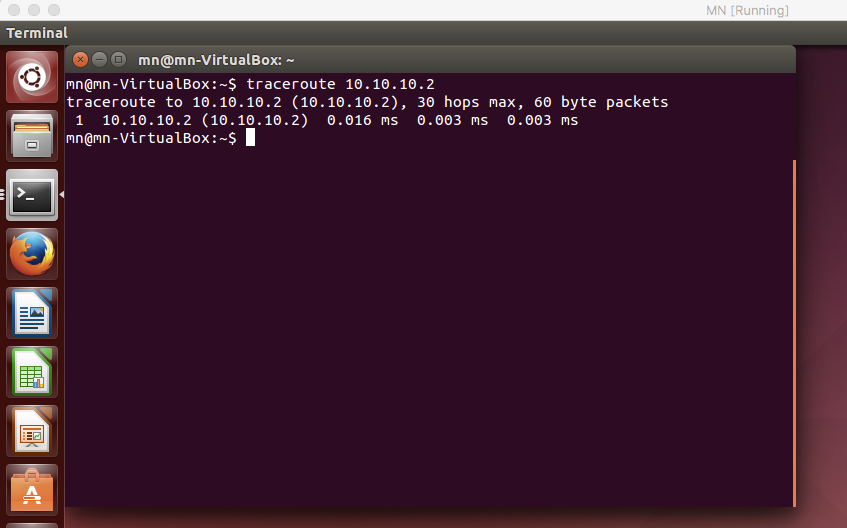
\includegraphics[width = 0.75\textwidth]{p1-img36}
 		\captionof{figure}{\label{fig:IPN}Estado de la aplicación web.} 
	\end{center} 
\end{figure}

Justo al lado de cada usuario de la lista, en la última columna de la tabla, aparece un botón titulado 'Borrar' que nos permite realizar la acción de eliminar el usuario de esa fila como se ve en la imagen. \\

\begin{figure}[H]
	\begin{center}
 		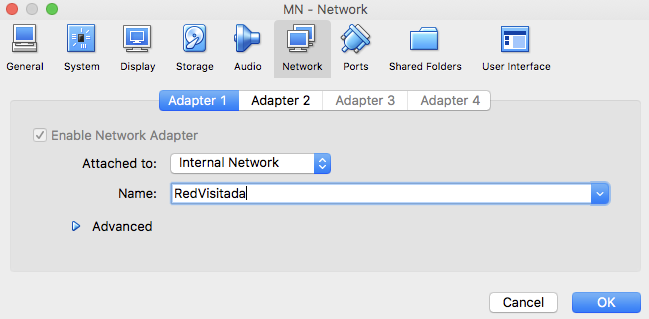
\includegraphics[width = 0.75\textwidth]{p1-img37}
 		\captionof{figure}{\label{fig:IPN}Acción de borrar en la aplicación web.} 
	\end{center} 
\end{figure}

Para hacer la prueba vamos a proceder a eliminar el último usuario de la lista para ver que efectivamente la lista ya muestra un usuario menos al ser eliminado de la base de datos.\\

\begin{figure}[H]
	\begin{center}
 		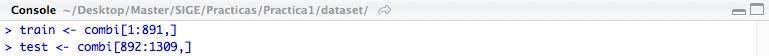
\includegraphics[width = 0.75\textwidth]{p1-img38}
 		\captionof{figure}{\label{fig:IPN}Borrar un usuario en la aplicación web (I).} 
	\end{center} 
\end{figure}

\begin{figure}[H]
	\begin{center}
 		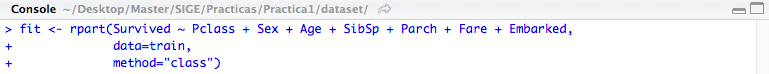
\includegraphics[width = 0.75\textwidth]{p1-img39}
 		\captionof{figure}{\label{fig:IPN}Borrar un usuario en la aplicación web (II).} 
	\end{center} 
\end{figure}

Vemos también como debajo de la tabla de los usuarios existe un formulario para poder registrar a un nuevo usuario en la aplicación. Este formulario solicita datos como el nombre (que es requerido), los apellidos y la edad. Si introducimos esos datos y pulsamos el botón titulado 'Insertar', veremos como la lista de los usuarios se actualiza con el nuevo registro insertado. \\

\begin{figure}[H]
	\begin{center}
 		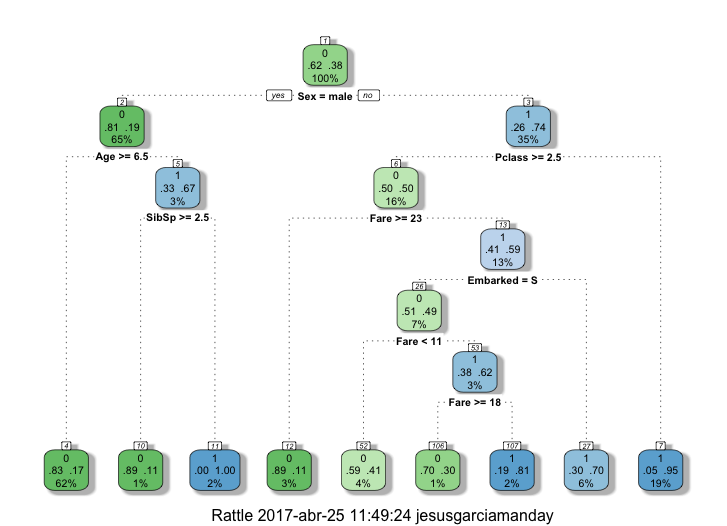
\includegraphics[width = 0.75\textwidth]{p1-img40}
 		\captionof{figure}{\label{fig:IPN}Insertar un usuario en la aplicación web (I).} 
	\end{center} 
\end{figure}

\begin{figure}[H]
	\begin{center}
 		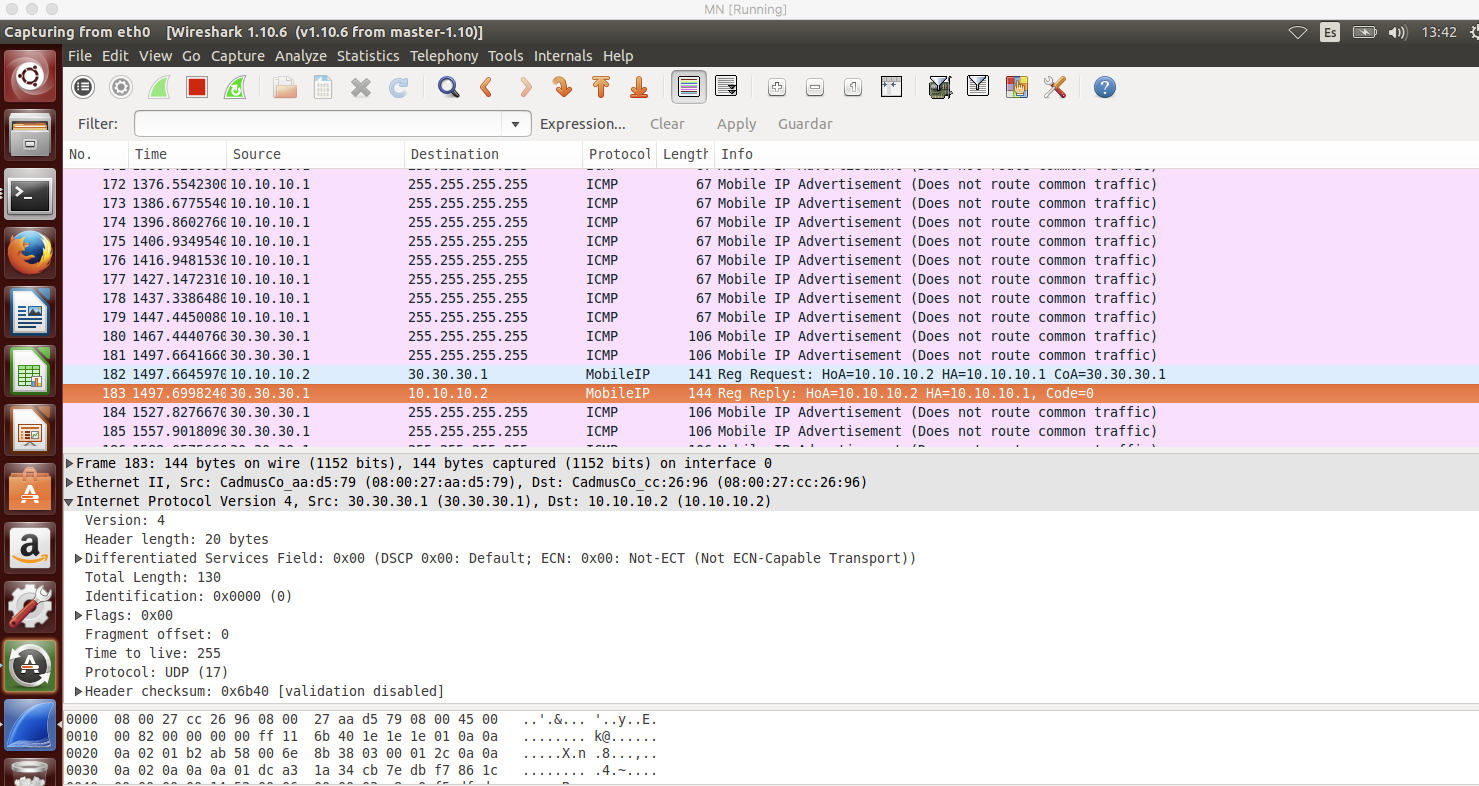
\includegraphics[width = 0.75\textwidth]{p1-img41}
 		\captionof{figure}{\label{fig:IPN}Insertar un usuario en la aplicación web (II).} 
	\end{center} 
\end{figure}


\section{Descripción del proceso de instalación del S.O. (desde una ISO) en la MV.}
El proceso de instalación de un sistema operativo desde una imagen ISO en una máquina virtual vamos a realizarlo desde el hipervisor \textbf{VirtualBox}. A través de este software interactivo basado en ventanas vamos a definir una máquina virtual e instalarle posteriormente el sistema operativo desde una image ISO. \\

La máquina virtual que se va a crear va a tener como sistema operativo un \textbf{Ubuntu} en la versión \textbf{14.04} de 64 bits y se llamará \textbf{vmUbuntu} como muestra la siguiente imagen. \\

\begin{figure}[H]
	\begin{center}
 		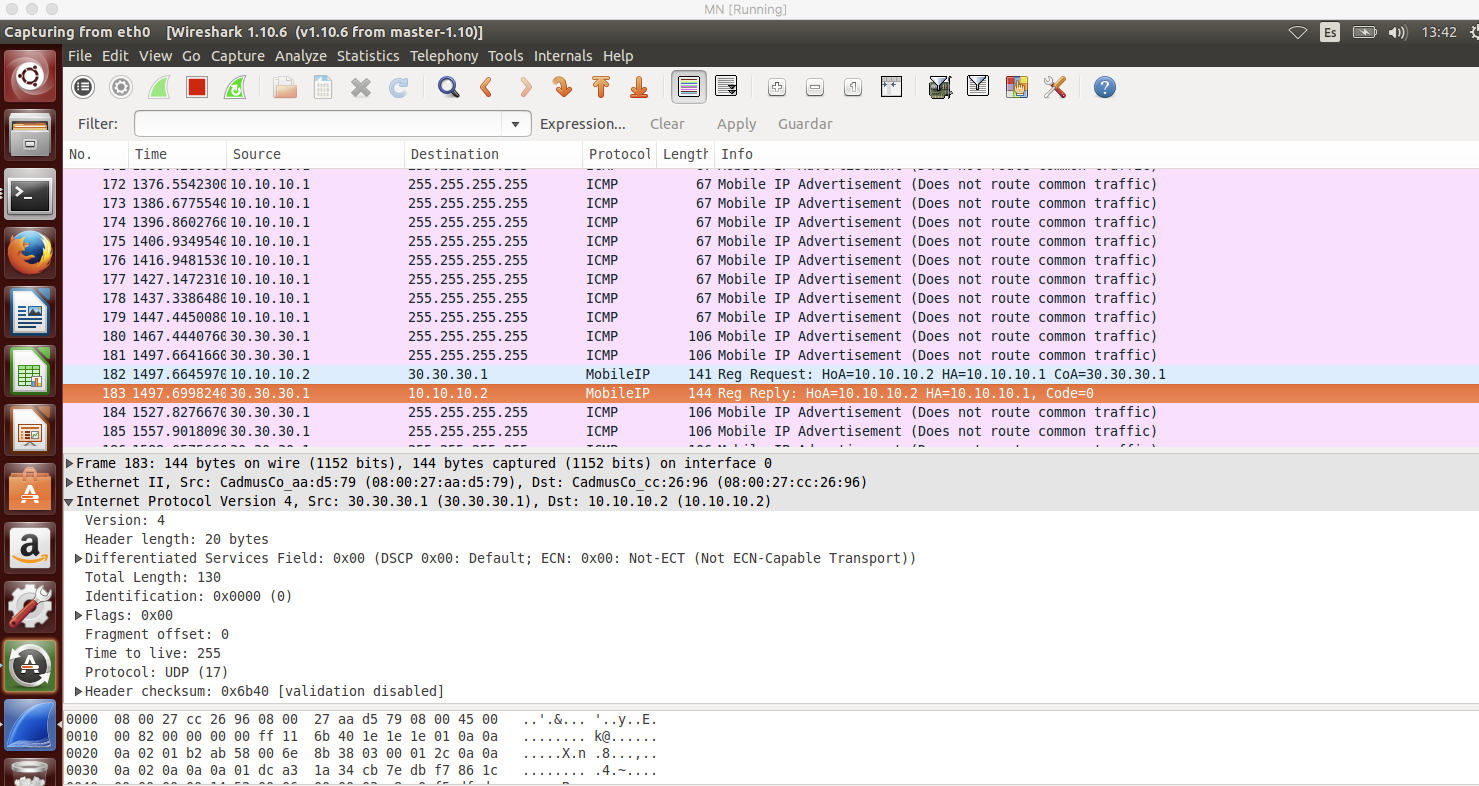
\includegraphics[width = 0.75\textwidth]{p1-img41}
 		\captionof{figure}{\label{fig:IPN}Creando máquina virtual (I).} 
	\end{center} 
\end{figure}
 
Se le asignará \textbf{1 GB} para el tamaño de memoria RAM, así como \textbf{8 GB} de tamaño de disco (el cual se creará) de tipo \textbf{VDI} y reservado dinámicamente. 

\begin{figure}[H]
	\begin{center}
 		
\includegraphics[width = 0.75\textwidth]{p1-img42}
 		\captionof{figure}{\label{fig:IPN}Creando máquina virtual (II).} 
	\end{center} 
\end{figure}

\begin{figure}[H]
	\begin{center}
 		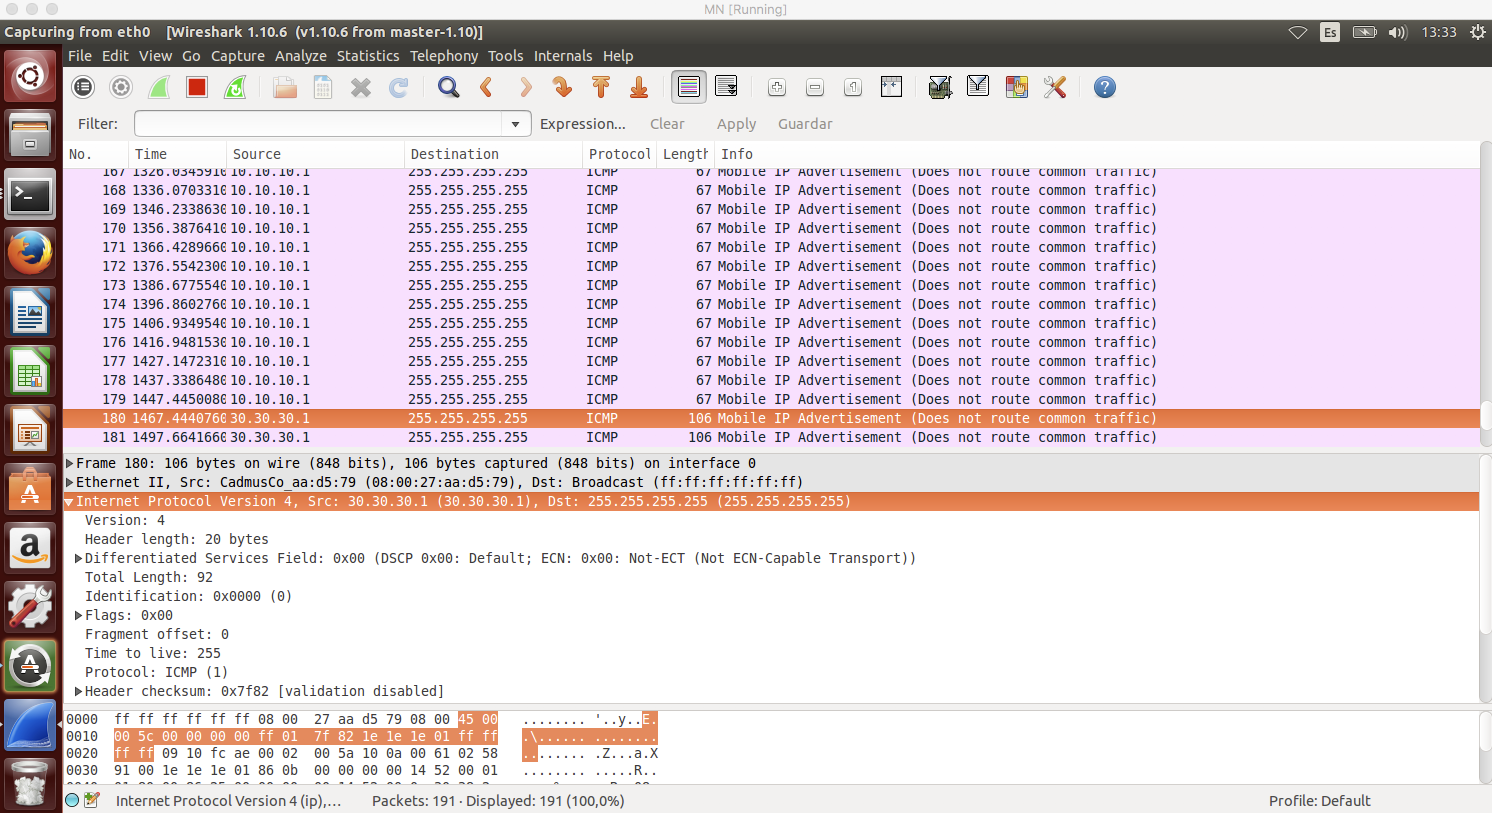
\includegraphics[width = 0.75\textwidth]{p1-img43}
 		\captionof{figure}{\label{fig:IPN}Creando máquina virtual (III).} 
	\end{center} 
\end{figure}

\begin{figure}[H]
	\begin{center}
 		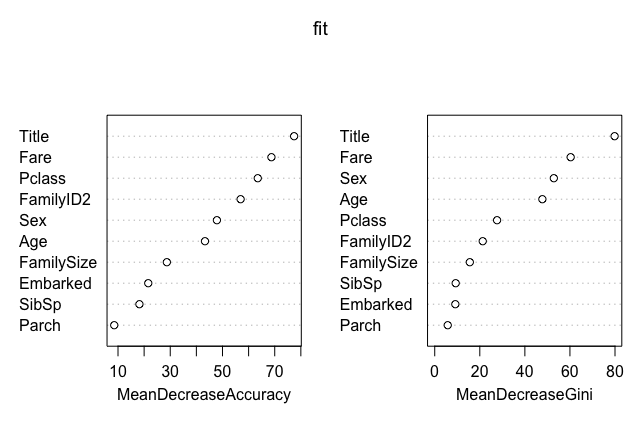
\includegraphics[width = 0.75\textwidth]{p1-img44}
 		\captionof{figure}{\label{fig:IPN}Creando máquina virtual (IV).} 
	\end{center} 
\end{figure}

\begin{figure}[H]
	\begin{center}
 		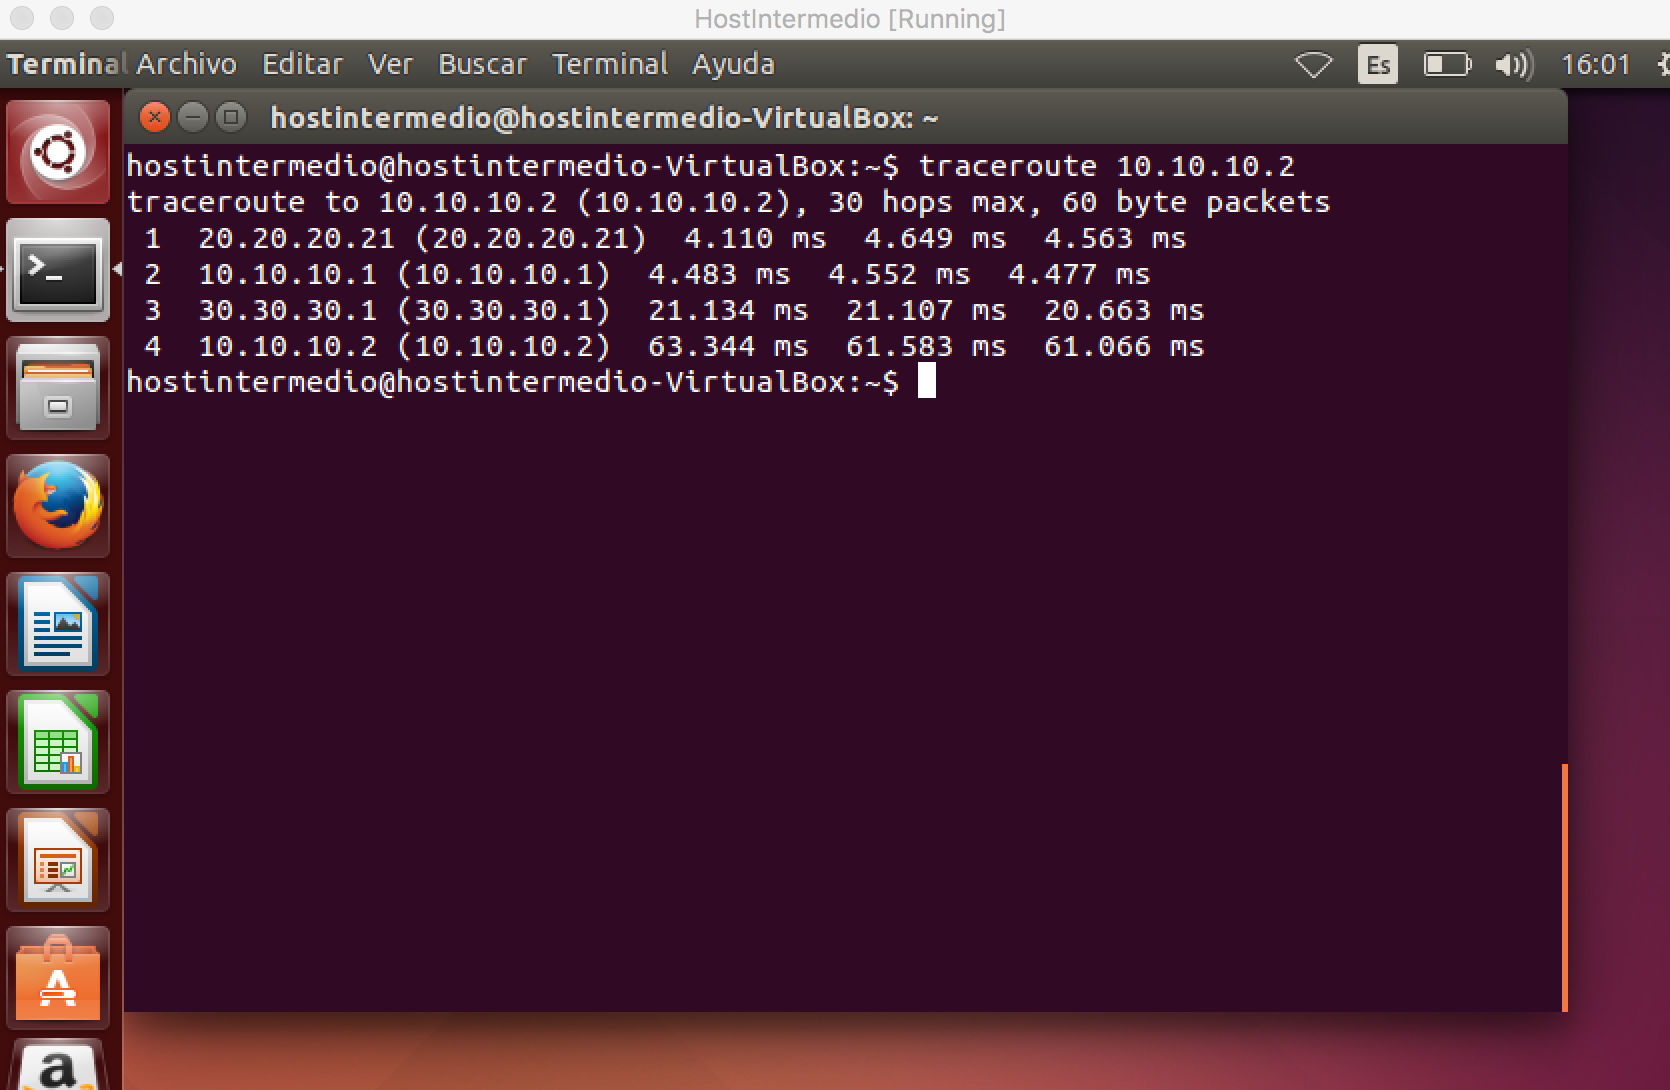
\includegraphics[width = 0.75\textwidth]{p1-img45}
 		\captionof{figure}{\label{fig:IPN}Creando máquina virtual (V).} 
	\end{center} 
\end{figure}

\begin{figure}[H]
	\begin{center}
 		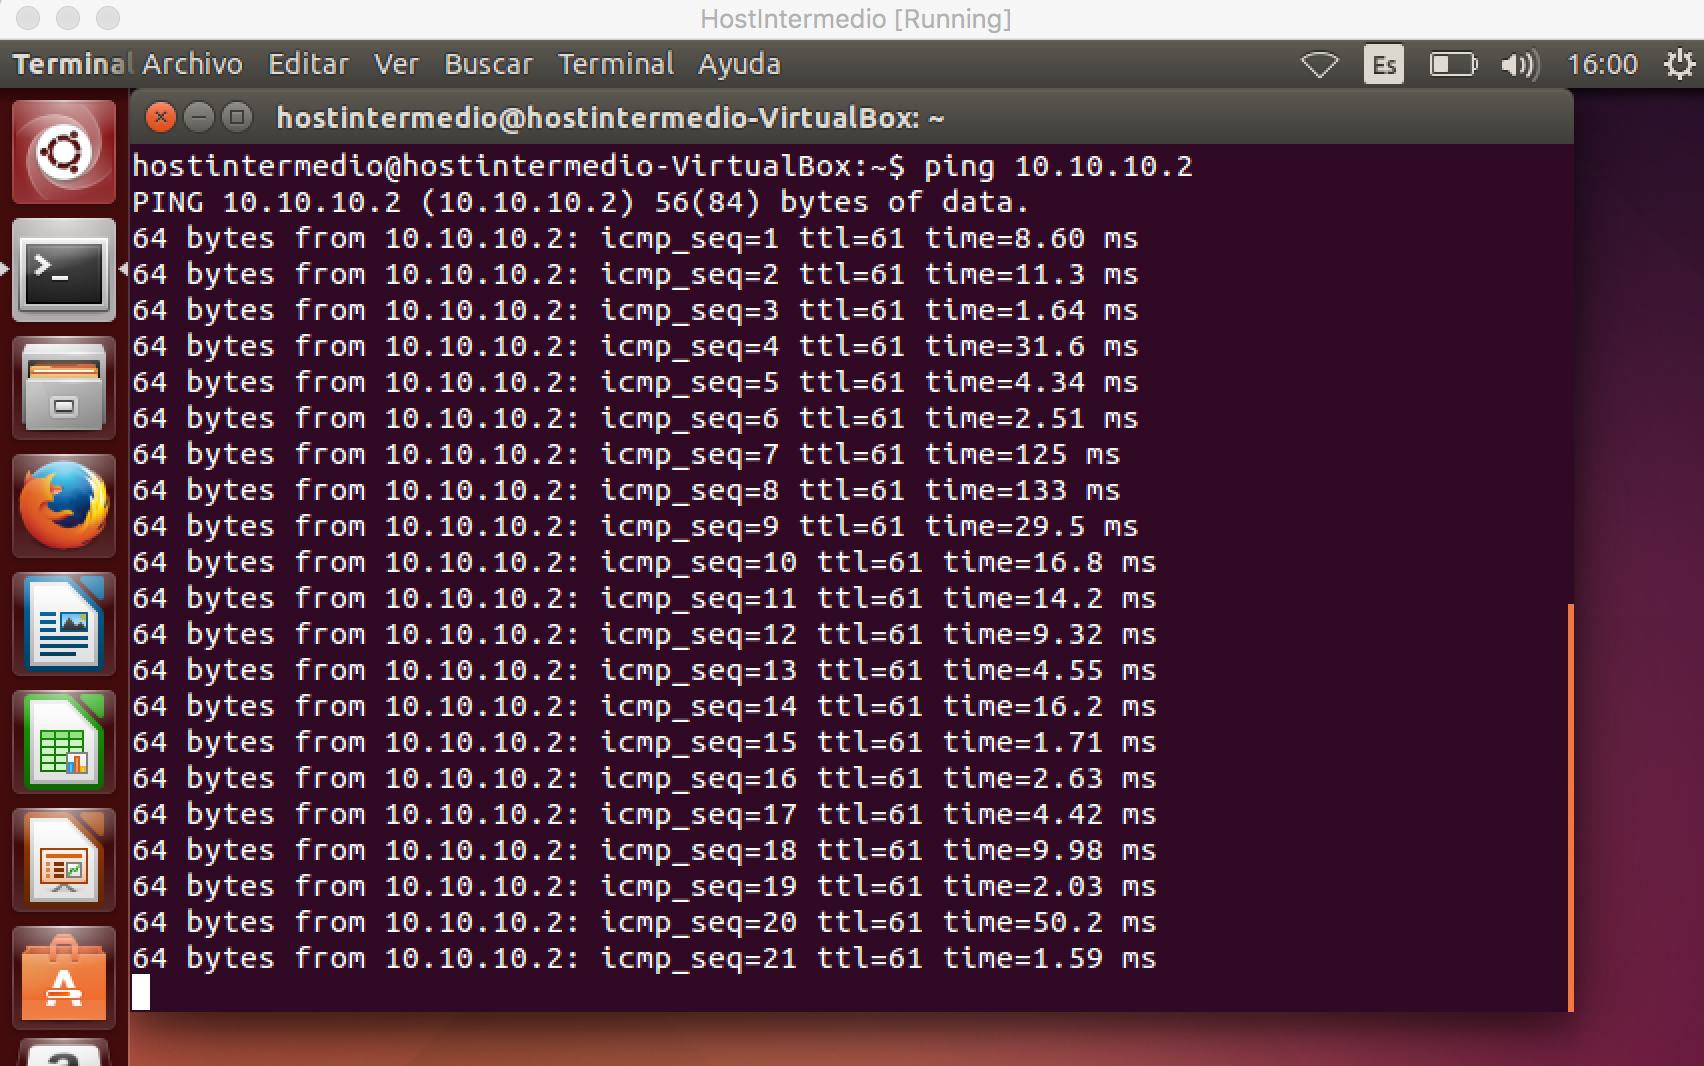
\includegraphics[width = 0.75\textwidth]{p1-img46}
 		\captionof{figure}{\label{fig:IPN}Creando máquina virtual (VI).} 
	\end{center} 
\end{figure}

\begin{figure}[H]
	\begin{center}
 		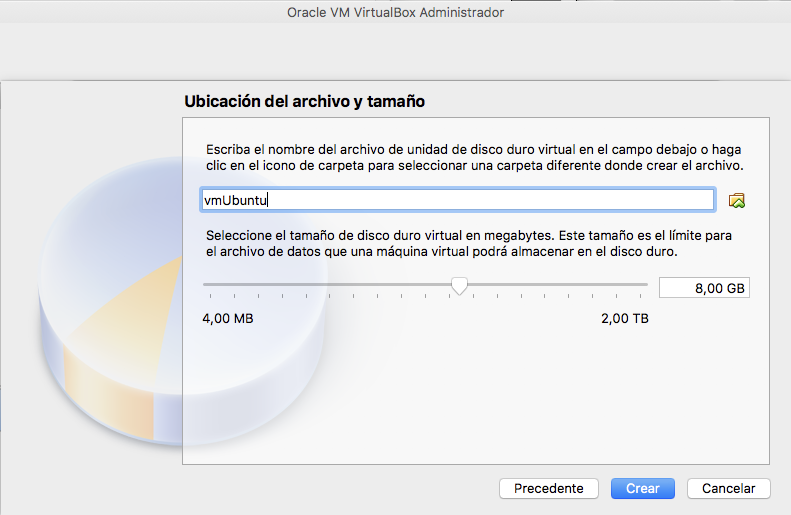
\includegraphics[width = 0.75\textwidth]{p1-img47}
 		\captionof{figure}{\label{fig:IPN}Creando máquina virtual (VII).} 
	\end{center} 
\end{figure}

Una vez que la máquina virtual ha sido creada, el siguiente paso es la instalación del sistema operativo, el cual será tomado desde una imagen ISO seleccionada.\\

\begin{figure}[H]
	\begin{center}
 		\includegraphics[width = 0.75\textwidth]{p1-img48}
 		\captionof{figure}{\label{fig:IPN}Máquina virtual creada.} 
	\end{center} 
\end{figure}

\begin{figure}[H]
	\begin{center}
 		\includegraphics[width = 0.75\textwidth]{p1-img49}
 		\captionof{figure}{\label{fig:IPN}Instalación del S.O desde una imagen ISO (I).} 
	\end{center} 
\end{figure}

\begin{figure}[H]
	\begin{center}
 		\includegraphics[width = 0.75\textwidth]{p1-img50}
 		\captionof{figure}{\label{fig:IPN}Instalación del S.O desde una imagen ISO (II).} 
	\end{center} 
\end{figure}

\begin{figure}[H]
	\begin{center}
 		\includegraphics[width = 0.75\textwidth]{p1-img51}
 		\captionof{figure}{\label{fig:IPN}Instalación del S.O desde una imagen ISO (III).} 
	\end{center} 
\end{figure}

\begin{figure}[H]
	\begin{center}
 		\includegraphics[width = 0.75\textwidth]{p1-img52}
 		\captionof{figure}{\label{fig:IPN}Instalación del S.O desde una imagen ISO (IV).} 
	\end{center} 
\end{figure}

\begin{figure}[H]
	\begin{center}
 		\includegraphics[width = 0.75\textwidth]{p1-img53}
 		\captionof{figure}{\label{fig:IPN}Instalación del S.O desde una imagen ISO (V).} 
	\end{center} 
\end{figure}

\begin{figure}[H]
	\begin{center}
 		\includegraphics[width = 0.75\textwidth]{p1-img54}
 		\captionof{figure}{\label{fig:IPN}Instalación del S.O desde una imagen ISO (VI).} 
	\end{center} 
\end{figure}

\begin{figure}[H]
	\begin{center}
 		\includegraphics[width = 0.75\textwidth]{p1-img55}
 		\captionof{figure}{\label{fig:IPN}Instalación del S.O desde una imagen ISO (VII).} 
	\end{center} 
\end{figure}

\begin{figure}[H]
	\begin{center}
 		\includegraphics[width = 0.75\textwidth]{p1-img56}
 		\captionof{figure}{\label{fig:IPN}Instalación del S.O desde una imagen ISO (VIII).} 
	\end{center} 
\end{figure}

\begin{figure}[H]
	\begin{center}
 		\includegraphics[width = 0.75\textwidth]{p1-img57}
 		\captionof{figure}{\label{fig:IPN}Instalación del S.O desde una imagen ISO (IX).} 
	\end{center} 
\end{figure}

\begin{figure}[H]
	\begin{center}
 		\includegraphics[width = 0.75\textwidth]{p1-img58}
 		\captionof{figure}{\label{fig:IPN}Instalación del S.O desde una imagen ISO (X).} 
	\end{center} 
\end{figure}

Como se ha podido ver en las imágenes la instalación del sistema operativo en la máquina virtual desde una imagen \textbf{ISO} se ha realizado correctamente paso por paso y dicha máquina ya se encuentra disponible para su uso. \\


\section{Descripción del proceso de instalación, configuración y despliegue de Owncloud.}
Owncloud es un servidor de ficheros compartidos open-source que permite almacenar contenido personal tales como documentos y fotografías en una localización centralizada. En este apartado se van a mostrar los pasos para su instalación, configuración y despliegue utilizando la máquina virtual creada en el apartado anterior. \\

La máquina donde se va a instalar este herramienta debe cumplir con una serie de requisitos necesarios tales como un servidor web (\textbf{Apache} para este caso, una base de datos \textbf{MySQL} y \textbf{PHP} correctamente funcionando, así que lo primero será instalar todas esas herramientas. \\

\begin{figure}[H]
	\begin{center}
 		\includegraphics[width = 0.75\textwidth]{p1-img59}
 		\captionof{figure}{\label{fig:IPN}Actualización del sistema.} 
	\end{center} 
\end{figure}

\begin{figure}[H]
	\begin{center}
 		\includegraphics[width = 0.75\textwidth]{p1-img60}
 		\captionof{figure}{\label{fig:IPN}Instalación de \textbf{Apache}.} 
	\end{center} 
\end{figure}

\begin{figure}[H]
	\begin{center}
 		\includegraphics[width = 0.75\textwidth]{p1-img61}
 		\captionof{figure}{\label{fig:IPN}Instalación de \textbf{PHP}.} 
	\end{center} 
\end{figure}

\begin{figure}[H]
	\begin{center}
 		\includegraphics[width = 0.75\textwidth]{p1-img62}
 		\captionof{figure}{\label{fig:IPN}Instalación de \textbf{MySQL}.} 
	\end{center} 
\end{figure}

Una vez instalados en la máquina virtual los requisitos necesarios para \textbf{Owncloud} pasamos a instalar la herramienta. Cabe indicar que no existe el paquete \textbf{Owncloud} dentro de los repositorios de Ubuntu, sino que mantiene su propio repositorio para la distribución, por lo que será necesarios descargar su \textbf{release key} y añadirlas con la utilidad \textbf{apt-key} para poder tener el fichero con la clave pública \textbf{PGP} que permita verificar la autenticidad del paquete \textbf{Owncloud}. \\

Realizando los siguientes pasos instalamos \textbf{Owncloud} en la máquina.\\

\begin{figure}[H]
	\begin{center}
 		\includegraphics[width = 0.75\textwidth]{p1-img63}
 		\captionof{figure}{\label{fig:IPN}Instalación de \textbf{Owncloud} (I).} 
	\end{center} 
\end{figure}

\begin{figure}[H]
	\begin{center}
 		\includegraphics[width = 0.75\textwidth]{p1-img64}
 		\captionof{figure}{\label{fig:IPN}Instalación de \textbf{Owncloud} (II).} 
	\end{center} 
\end{figure}

\begin{figure}[H]
	\begin{center}
 		\includegraphics[width = 0.75\textwidth]{p1-img65}
 		\captionof{figure}{\label{fig:IPN}Instalación de \textbf{Owncloud} (III).} 
	\end{center} 
\end{figure}

\begin{figure}[H]
	\begin{center}
 		\includegraphics[width = 0.75\textwidth]{p1-img66}
 		\captionof{figure}{\label{fig:IPN}Instalación de \textbf{Owncloud} (IV).} 
	\end{center} 
\end{figure}

Con el paquete \textbf{Owncloud} instalado en la máquina virtual, el siguiente paso es configurar la base de datos \textbf{MySQL}. Es necesario crear una base de datos separada donde \textbf{Owncloud} almacenará los datos administrativos.\\

\begin{figure}[H]
	\begin{center}
 		\includegraphics[width = 0.75\textwidth]{p1-img67}
 		\captionof{figure}{\label{fig:IPN}Configurando \textbf{Owncloud} (I).} 
	\end{center} 
\end{figure}

Crearemos también una cuenta de usuario \textbf{MySQL} que interactuará con la base de datos creada anteriormente, siendo este el que la manejará.\\

\begin{figure}[H]
	\begin{center}
 		\includegraphics[width = 0.75\textwidth]{p1-img68}
 		\captionof{figure}{\label{fig:IPN}Configurando \textbf{Owncloud} (II).} 
	\end{center} 
\end{figure}

Ya podemos desplegar el servidor \textbf{Owncloud} una vez que hemos finalizado la configuración. Para probar su funcionamiento accedemos desde el navegador a la dirección \textbf{http:localhost:owncloud}, accedemos dando las credenciales para una nueva cuenta de administrador y ya podemos comenzar a almacenar datos en nuestro servidor.\\

\begin{figure}[H]
	\begin{center}
 		\includegraphics[width = 0.75\textwidth]{p1-img69}
 		\captionof{figure}{\label{fig:IPN}Desplegando \textbf{Owncloud} (I).} 
	\end{center} 
\end{figure}

\begin{figure}[H]
	\begin{center}
 		\includegraphics[width = 0.75\textwidth]{p1-img70}
 		\captionof{figure}{\label{fig:IPN}Desplegando \textbf{Owncloud} (II).} 
	\end{center} 
\end{figure}


\begin{figure}[H]
	\begin{center}
 		\includegraphics[width = 0.75\textwidth]{p1-img71}
 		\captionof{figure}{\label{fig:IPN}Desplegando \textbf{Owncloud} (III).} 
	\end{center} 
\end{figure}


\section{Referencias.}
\begin{itemize}
	\item \href{https://www.digitalocean.com/community/tutorials/how-to-install-and-configure-owncloud-on-ubuntu-16-04}{Instalación, configuración y despliegue de Owncloud}
\end{itemize}



\end{document}